\title{\color{ladrillo}\bfseries Romanos 11: la restauración de Israel\\[4pt]\large\color{cafe}\mdseries Dios no ha desechado a su pueblo: del remanente presente a la salvación de «todo Israel»}
\author{}\date{\color{sepia}Serie «Israel, el pueblo de Dios» · Estudio 8}
\begin{document}
\maketitle\thispagestyle{empty}

\begin{abstract}\noindent
Este estudio final de la serie analiza Romanos 11 en sus dimensiones histórica, literaria, filológica y teológica, y muestra que el capítulo responde con un «de ningún modo» a la pregunta de si Dios desechó a su pueblo. Defiende dos tesis que recogen los hilos de los siete estudios anteriores. Primera: la vocación de Israel como pueblo escogido, «reino de sacerdotes y nación santa» (Éx 19:6), no fue revocada por la incredulidad de la mayoría; se preserva en un remanente escogido por gracia y se proyecta hacia una plenitud futura, porque «irrevocables son los dones y el llamamiento de Dios» (Ro 11:29). Segunda: la promesa de restauración que recorre la historia de Israel (Gn 15; Dt 30; Is 59; Jer 31; Ez 37) alcanza en Ro 11:25--27 su formulación más explícita en el Nuevo Testamento: un endurecimiento parcial y temporal, la entrada de la plenitud de las naciones y la salvación de «todo Israel» cuando el Redentor quite la impiedad de Jacob. El estudio sitúa la carta en la comunidad de Roma después del edicto de Claudio, analiza la estructura de Ro 9--11 y el uso de las citas del Antiguo Testamento según el Texto Masorético y la Septuaginta, estudia el vocabulario griego clave (\emph{pṓrōsis}, \emph{plḗrōma}, \emph{mystḗrion}, \emph{kaì hoútōs}, \emph{pâs Israḗl}), evalúa las principales interpretaciones de «todo Israel» con autores de cada postura e incorpora la tradición judía. Concluye que la lectura más consistente con el contexto de Ro 11 es la restauración futura del Israel étnico como conjunto que reconocerá al Mesías, sin que ello implique la salvación de cada individuo ni una salvación por linaje sin fe.
\par\smallskip\noindent\textbf{Palabras clave:} Romanos 11, todo Israel, remanente, endurecimiento, plenitud de los gentiles, olivo, nuevo pacto, restauración.
\end{abstract}

\section{Introducción}

«Digo, pues: ¿Ha desechado Dios a su pueblo? ¡De ningún modo!» (Ro 11:1). La pregunta de Pablo no es retórica en el sentido de ociosa. Hacia el año 57 e.\,c., la mayoría del pueblo judío no había reconocido a Jesús como Mesías, mientras que en las sinagogas y casas de Roma crecía el número de creyentes de las naciones. Un lector de esas iglesias podía sacar una conclusión rápida: Dios cambió de pueblo. Pablo dedica tres capítulos (Ro 9--11) a desmontar esa conclusión, y el capítulo 11 contiene su respuesta final.

Este estudio cierra la serie porque Ro 11 reúne todas sus piezas. Pablo se presenta como israelita, «de la descendencia de Abraham, de la tribu de Benjamín» (11:1; Estudios 1 y 3); recurre a Elías y a los siete mil que no doblaron la rodilla ante Baal, en el reino del norte (11:2--4; Estudio 5); cita a Moisés y a Isaías sobre el endurecimiento (11:8; Estudios 2 y 5); llama a David como testigo (11:9; Estudio 4); habla de raíz santa, primicias y ramas (11:16; Estudio 1); anuncia que el Redentor vendrá de Sion y que el pacto quitará los pecados de Jacob (11:26--27; Estudios 5 y 6); y escribe con la experiencia de una Jerusalén que todavía tenía templo, pero cuya caída Jesús ya había anunciado (Lc 21:24; Estudio 7).

La tesis es doble, como en toda la serie:
\begin{enumerate}
\item \textbf{Identidad y vocación.} Israel sigue siendo el pueblo que Dios «conoció de antemano» (11:2). Su vocación de «reino de sacerdotes y nación santa» no fue anulada por la incredulidad de la mayoría: se preserva en un remanente escogido por gracia (11:5) y alcanzará su plenitud (11:12), porque el llamamiento de Dios es irrevocable (11:29).
\item \textbf{Promesa de restauración.} Ro 11:25--27 es el punto de llegada de la promesa renovada en cada etapa: el endurecimiento es parcial y tiene un límite («hasta que»), y después «todo Israel será salvo», según el pacto anunciado por Isaías y Jeremías.
\end{enumerate}

\begin{center}\small
\renewcommand{\arraystretch}{1.3}
\begin{tabular}{>{\RaggedRight\arraybackslash}p{2.4cm}>{\RaggedRight\arraybackslash}p{6.4cm}>{\RaggedRight\arraybackslash}p{5.2cm}}
\toprule
\textbf{Dimensión} & \textbf{Pregunta que formula} & \textbf{Textos y fuentes}\\
\midrule
Histórica & ¿Qué situación de Roma y de Israel explica que Pablo escriba Ro 11? & Hch 18:2; 21:20; Ro 15:25--27; 16:3--5; Suetonio, \emph{Claudio} 25.4\\
Literaria & ¿Cómo está construido el argumento de Ro 9--11 y qué función tienen sus citas y metáforas? & Ro 9:1--5; 11:1--36; citas de 1~R, Dt, Is, Sal, Jer, Job\\
Filológica & ¿Qué dicen exactamente las palabras griegas clave y cómo reflejan el hebreo y la Septuaginta? & NA28; BHS; Rahlfs-Hanhart\\
Teológica & ¿Qué afirma el capítulo sobre la elección, el remanente, el endurecimiento y la salvación de Israel? & Ro 11:1--2, 5, 11--12, 15, 23, 25--32\\
\bottomrule
\end{tabular}\end{center}

Las cuatro dimensiones no son compartimentos: el contexto histórico explica el tono de advertencia a los gentiles; la forma literaria marca dónde está el clímax; la filología decide qué significa «y así»; y la teología recoge todo en una afirmación sobre la fidelidad de Dios. Después del análisis, el estudio expone las interpretaciones de «todo Israel» con sus autores, traza los hilos de la serie que confluyen en Ro 11, recoge la tradición judía y extrae implicaciones.

\begin{nota}[Sobre traducción, numeración, fechas y el nombre «Israel»]
Las citas bíblicas son traducción propia desde el texto hebreo (BHS) y griego (NA28); la Septuaginta (LXX) se cita según Rahlfs-Hanhart. Cuando la numeración hebrea o griega difiere de la española, se da la española y entre corchetes la otra, por ejemplo Sal 69:22 [69:23; LXX 68:23]. Las fechas se indican como a.\,e.\,c. y e.\,c. En Ro 9--11, «Israel» (\grc{Ἰσραήλ}) designa siempre al pueblo completo, descendiente de Jacob, y nunca al antiguo reino del norte; cuando este estudio se refiera al reino del norte (Efraín, Samaria) o al reino del sur (Judá, Jerusalén), lo dirá explícitamente.
\end{nota}

\section{Dimensión histórica}

\subsection{Marco cronológico}
Romanos es la carta de Pablo que mejor se puede fechar. Pablo escribe cuando está a punto de llevar a Jerusalén la colecta de las iglesias de Macedonia y Acaya (Ro 15:25--26), es decir, al final de los tres meses que pasa en Grecia según Hch 20:2--3. Recomienda a Febe, «diaconisa de la iglesia en Cencrea», el puerto oriental de Corinto (Ro 16:1), y envía saludos de Gayo, que lo hospeda, y de Erasto, «tesorero de la ciudad» (16:23). La mayoría de los comentaristas sitúan la carta en Corinto entre el 55 y el 58 e.\,c., con preferencia por el invierno del 56--57 (Cranfield, 1975; Moo, 1996; Fitzmyer, 1993; Jewett, 2007).

\begin{center}\begin{minipage}{\linewidth}\centering
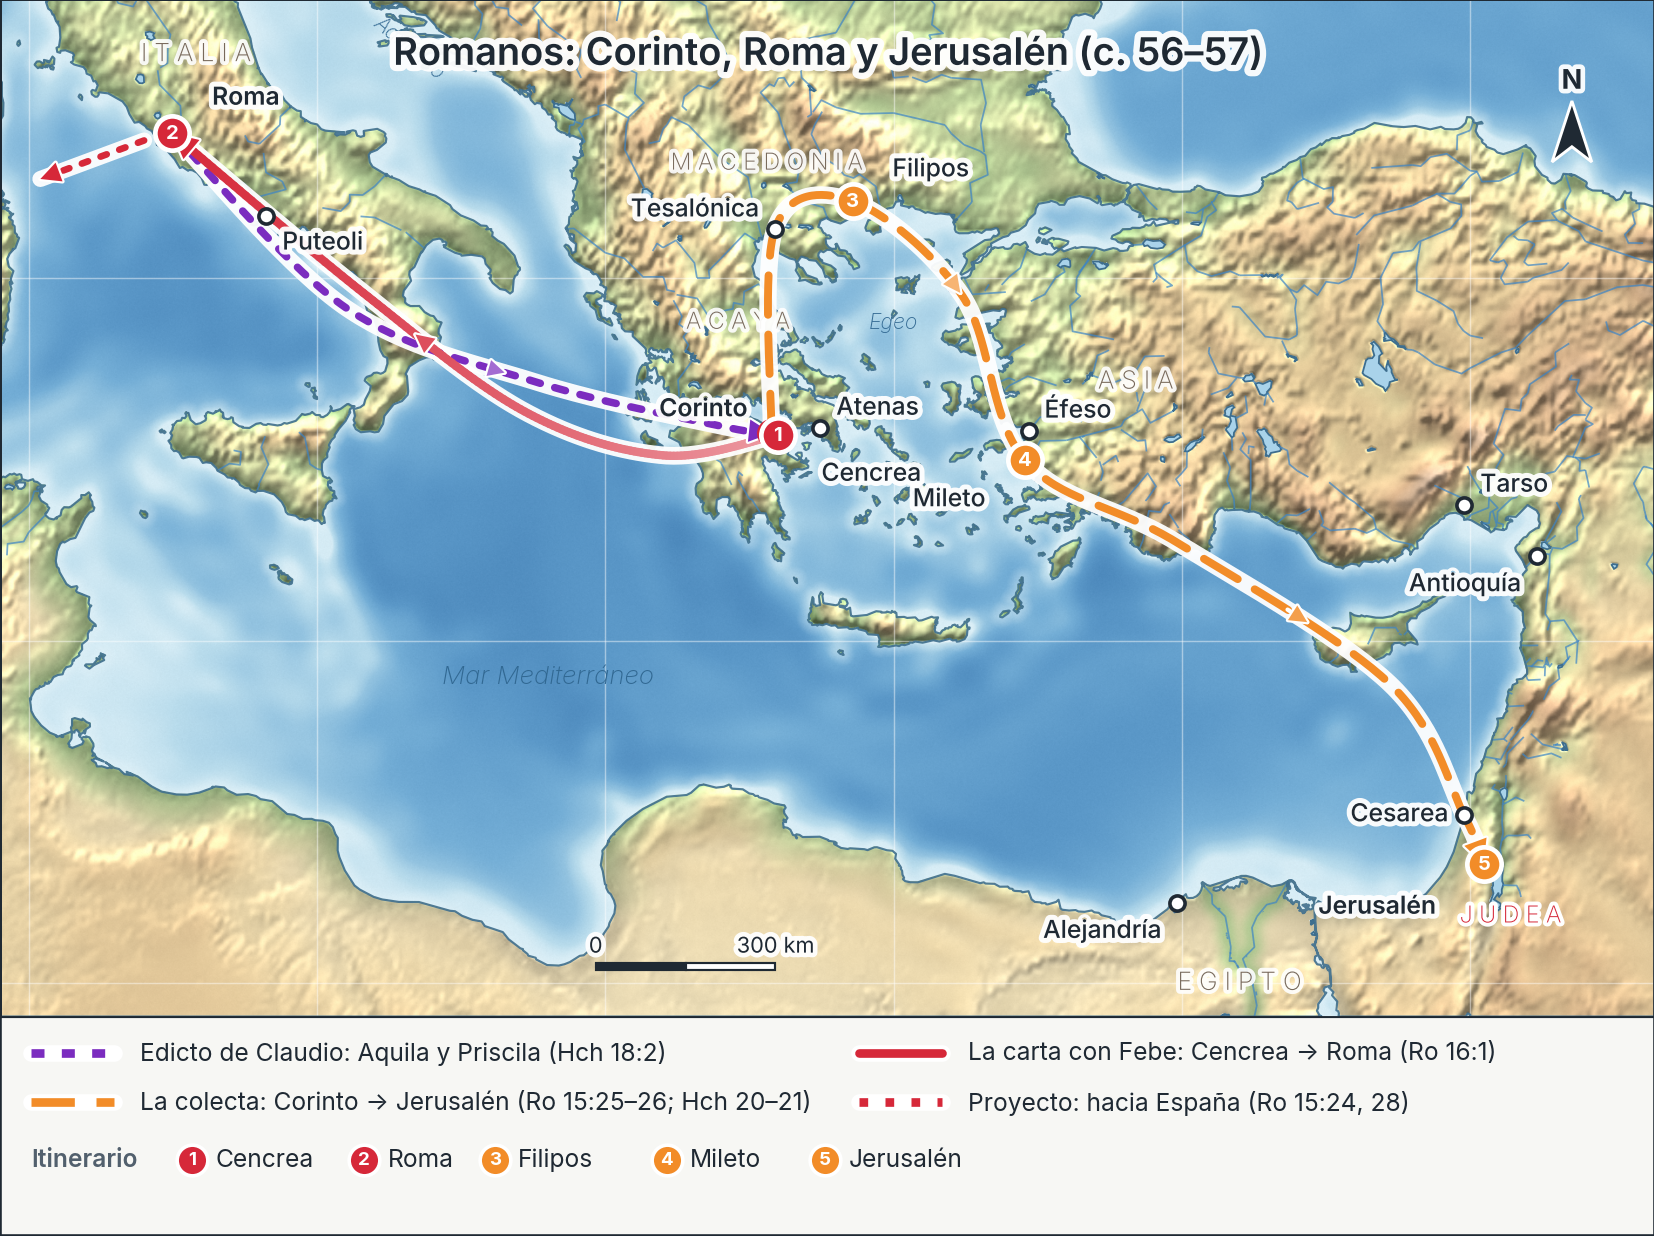
\includegraphics[width=1\linewidth]{mapa_romanos.png}\\[2pt]
{\footnotesize\color{sepia}\textit{Nota.} Elaboración propia: costas, lagos y ríos GSHHS/WDB y relieve sombreado (Basemap); ubicaciones antiguas aproximadas. }
\end{minipage}\end{center}


\begin{center}\begin{minipage}{\linewidth}\centering
\begin{tikzpicture}[x=1cm,y=1cm]
\draw[line width=1.6pt,cafe,-{Latex[length=3mm]}] (0,0) -- (15.6,0);
\foreach \x/\t/\b in {0.5/{Pompeyo toma Jerusalén}/{63 a.\,e.\,c.; cautivos a Roma},
                      2.2/{Expulsión bajo Tiberio}/{19 e.\,c.; Josefo, \emph{Ant.} 18.81--84},
                      3.9/{Edicto de Claudio}/{c. 49; Suetonio; Hch 18:2},
                      5.6/{Pablo en Corinto}/{c. 50--52; Hch 18:1--11},
                      7.3/{Muere Claudio}/{54; regreso de judíos (Ro 16:3)},
                      9.0/{Carta a los Romanos}/{c. 56--57, desde Corinto},
                      10.7/{Colecta y arresto}/{c. 57; Hch 21},
                      12.4/{Persecución de Nerón}/{64; Tácito, \emph{Ann.} 15.44},
                      14.1/{Caída del templo}/{70 (Estudio 7)}}{
  \fill[oro] (\x,0) circle (4pt);
  \node[above,font=\scriptsize\bfseries,text=ladrillo,text width=1.6cm,align=center] at (\x,0.2) {\t};
  \node[below,font=\tiny,text=sepia,text width=1.6cm,align=center] at (\x,-0.2) {\b};}
\draw[decorate,decoration={brace,amplitude=5pt,mirror},sepia] (3.6,-1.15) -- (7.6,-1.15) node[midway,below=5pt,font=\scriptsize\itshape]{Expulsión y regreso};
\draw[decorate,decoration={brace,amplitude=5pt,mirror},sepia] (8.7,-1.15) -- (11.0,-1.15) node[midway,below=5pt,font=\scriptsize\itshape]{Ro 15:25--32};
\end{tikzpicture}\par\smallskip
{\footnotesize\color{sepia}\textit{Nota.} Elaboración propia. Las fechas del edicto de Claudio y de la carta son aproximadas (véase el texto).}
\end{minipage}\end{center}

\begin{nota}[Precisión arqueológica: Galión y Erasto]
Dos inscripciones reales ayudan a fechar y a situar la carta, con distinto grado de certeza. La \textbf{inscripción de Galión}, hallada en Delfos, reproduce una carta del emperador Claudio que menciona a Junio Galión como procónsul de Acaya; permite fechar su proconsulado hacia el 51--52 e.\,c. y, con él, la estancia de Pablo en Corinto de Hch 18:12. La \textbf{inscripción de Erasto}, en un pavimento cercano al teatro de Corinto, dice que Erasto costeó el pavimento a cambio de su cargo de edil. Muchos la relacionan con el «Erasto, tesorero de la ciudad» de Ro 16:23, pero la identificación está en debate: el título griego (\grc{οἰκονόμος τῆς πόλεως}) no coincide exactamente con el latino (\emph{aedilis}), y la fecha del pavimento se discute.
\end{nota}

\subsection{Los judíos en Roma}
Había una comunidad judía en Roma al menos desde el siglo \textsc{ii} a.\,e.\,c., y creció cuando Pompeyo llevó cautivos judíos tras tomar Jerusalén en el 63 a.\,e.\,c. Filón cuenta que muchos de ellos, luego liberados, vivían al otro lado del Tíber (\emph{Legatio ad Gaium} 155--157), y Cicerón ya alude a su número e influencia en el 59 a.\,e.\,c. (\emph{Pro Flacco} 66). Las inscripciones de las catacumbas judías de Roma (Monteverde, Vigna Randanini, Villa Torlonia) nombran varias sinagogas independientes, como la de los «Augustenses», los «Agripenses» o los «Hebreos» (Leon, 1960). No había una autoridad central: cada sinagoga era una comunidad propia. La población judía de la ciudad se estima entre 20\,000 y 50\,000 personas, una cifra incierta.

Ese tejido explica cómo llegó el evangelio a Roma. Nadie sabe quién lo llevó. Hch 2:10 menciona «romanos residentes, tanto judíos como prosélitos» presentes en Pentecostés, y un comentarista latino del siglo \textsc{iv}, conocido como Ambrosiáster, escribe que los romanos habían recibido la fe «según el rito judío», sin haber visto milagros ni apóstoles (prólogo a Romanos). Lo probable es que el mensaje sobre Jesús circulara primero dentro de las sinagogas, entre judíos y entre los gentiles «temerosos de Dios» que asistían a ellas.

\subsection{El edicto de Claudio}
El historiador Suetonio, a comienzos del siglo \textsc{ii}, escribe en su vida de Claudio:
\begin{cita}A los judíos, que provocaban continuos tumultos por instigación de Cresto, los expulsó de Roma.\fuente{(Suetonio, \emph{Claudio} 25.4: \emph{Iudaeos impulsore Chresto assidue tumultuantis Roma expulit})}\end{cita}
Hch 18:2 confirma una expulsión: Pablo encuentra en Corinto a Aquila y Priscila, «recién venidos de Italia, porque Claudio había mandado que todos los judíos salieran de Roma». La mayoría de los historiadores entiende que «Cresto» es una forma de \emph{Christus}, frecuente porque en la pronunciación de la época \emph{Chrestus} (nombre común de esclavos, «útil») y \emph{Christus} sonaban casi igual. Si es así, los «tumultos» fueron conflictos dentro de las sinagogas por la predicación de Jesús como Mesías, y Suetonio confundió el objeto de la disputa con un agitador presente. Otros piensan que Cresto era un judío romano real con ese nombre. El dato es probable, no seguro.

La fecha también se discute. Orosio, en el siglo \textsc{v}, sitúa el edicto en el noveno año de Claudio, el 49 e.\,c. (\emph{Historias} 7.6.15), y dice tomar el dato de Josefo, aunque no aparece en las obras conservadas de Josefo. Dión Casio cuenta que Claudio, al comienzo de su reinado (41 e.\,c.), no expulsó a los judíos porque eran demasiados, pero les prohibió reunirse (\emph{Historia romana} 60.6.6). Algunos autores piensan que hubo dos medidas distintas; otros, que Dión y Suetonio describen la misma. La fecha del 49 encaja bien con Hch 18 y con la cronología de Galión, y es la que sigue la mayoría.

Lo importante para Ro 11 es la consecuencia. Si los judíos, incluidos los judíos creyentes en Jesús como Aquila y Priscila, debieron salir de Roma, las asambleas cristianas quedaron durante unos años formadas casi solo por gentiles. Cuando Claudio murió en el 54 y el edicto perdió vigencia, los judíos volvieron: en Ro 16:3--5 Priscila y Aquila ya están de regreso, con una iglesia en su casa. Wiefel (1991) propuso que esa secuencia explica la carta: los judíos creyentes regresaban a comunidades ahora dirigidas por gentiles, que se habían acostumbrado a vivir sin ellos y empezaban a considerarlos un pueblo descartado. La hipótesis es discutida en sus detalles, pero describe con precisión el problema que Pablo enfrenta en Ro 11:13--25.

\subsection{La colecta para Jerusalén}
Pablo escribe a Roma camino de Jerusalén:
\begin{cita}Pero ahora voy a Jerusalén para servir a los santos. Porque Macedonia y Acaya tuvieron a bien hacer una colecta para los pobres de entre los santos que están en Jerusalén. Les pareció bien, y son deudores de ellos; porque si los gentiles han sido hechos participantes de sus bienes espirituales, deben también servirles con los materiales.\fuente{(Ro 15:25--27)}\end{cita}
El razonamiento anticipa el olivo de Ro 11: los gentiles son \emph{participantes} (\grc{ἐκοινώνησαν}) de los bienes espirituales de los judíos, como en 11:17 son «copartícipes» (\grc{συγκοινωνός}) de la raíz del olivo. La colecta (1~Co 16:1--4; 2~Co 8--9; Gá 2:10) es la forma material de esa deuda. Pablo teme que no sea aceptada y pide oración (Ro 15:30--31). Cuando llega a Jerusalén, Santiago y los ancianos le dicen: «Ya ves, hermano, cuántas miríadas de judíos hay que han creído, y todos son celosos de la ley» (\grc{πόσαι μυριάδες εἰσὶν ἐν τοῖς Ἰουδαίοις τῶν πεπιστευκότων}, Hch 21:20). Ese es el «remanente escogido por gracia» de Ro 11:5: no un puñado simbólico, sino una comunidad numerosa en Jerusalén y Judea que seguía viviendo como judía.

\subsection{Fuertes y débiles}
En Ro 14:1--15:13 Pablo trata un conflicto entre los «fuertes», que comen de todo y no distinguen días, y los «débiles», que se abstienen de ciertos alimentos y guardan días. No dice que los débiles sean judíos ni que los fuertes sean gentiles, pero las categorías («puro» e «impuro», \grc{κοινός}, 14:14; observancia de días, 14:5--6) remiten a la práctica judía. Pablo pide a ambos grupos que se reciban mutuamente y cierra con una cadena de citas sobre las naciones que alaban con Israel (15:9--12), la última de Is 11:10: «Estará la raíz de Isaí, y el que se levantará a gobernar las naciones; en él esperarán las naciones» (15:12). La «raíz» davídica de Ro 15:12 completa la «raíz» del olivo de Ro 11:16--18.

\subsection{La arrogancia gentil que Pablo corrige}
Ro 11:13 marca un cambio de destinatario: «A vosotros hablo, gentiles». Desde ahí hasta 11:32, Pablo se dirige en segunda persona a creyentes de las naciones. Las advertencias son directas: «no te jactes contra las ramas» (11:18); «no te ensoberbezcas, sino teme» (11:20); «para que no seáis sabios en vuestra propia opinión» (11:25). Estas frases suponen un problema real en Roma: creyentes gentiles que veían la incredulidad de la mayoría de Israel como prueba de que Dios había pasado a ellos. Romanos 11 es, por tanto, una corrección pastoral además de un tratado teológico. Pablo no escribe para satisfacer la curiosidad escatológica, sino para impedir que la iglesia de las naciones se construya sobre el desprecio a Israel.

\subsection{Israel en tiempos de Pablo}
El panorama del pueblo judío hacia el 57 e.\,c. tenía tres rasgos que Ro 11 refleja:
\begin{itemize}
\item \textbf{Un remanente creyente visible}, con centro en Jerusalén y dirigido por Santiago, hermano del Señor (Gá 1:19; 2:9; Hch 15; 21:18--20), además de judíos creyentes en la diáspora como Pablo, Bernabé, Aquila, Priscila, Andrónico y Junia, a quienes Pablo llama «mis parientes» (Ro 16:7).
\item \textbf{Una mayoría que no creía}, por la que Pablo siente «gran tristeza y continuo dolor» (Ro 9:2) y por cuya salvación ora (10:1).
\item \textbf{Una tensión creciente con Roma} que desembocará en la guerra del 66--70 y en la destrucción del templo (Estudio 7). Pablo no la menciona, pero escribe a la capital del imperio que destruirá Jerusalén trece años después.
\end{itemize}

\subsection{Romanos leída en contexto judío}
Durante siglos Romanos se leyó como un tratado sobre la justificación individual en el que los capítulos 9--11 eran un paréntesis. El siglo \textsc{xx} cambió esa lectura. Stendahl (1976) sostuvo que Ro 9--11 no es un apéndice sino el clímax de la carta, cuyo tema es la relación entre judíos y gentiles en el plan de Dios. Sanders (1977) mostró que el judaísmo del Segundo Templo no era una religión de mérito, sino de pacto. Nanos (1996) propuso leer la carta como dirigida a creyentes gentiles que todavía se reunían en el ámbito de las sinagogas romanas, y entendió a los «débiles» de Ro 14 como judíos no creyentes en Jesús. Das (2007) defendió que los destinatarios explícitos son gentiles, aunque la comunidad incluyera judíos. Estas propuestas no coinciden entre sí, pero comparten un punto que este estudio adopta: \destacar{Ro 11 no es un desvío, sino la meta del argumento de la carta}, anunciada ya en su tema: el evangelio es poder de Dios para salvación «al judío primeramente, y también al griego» (Ro 1:16).

\begin{nota}[Precisión: el «debate sobre Romanos»]
Bajo el nombre de \emph{The Romans Debate} (Donfried, 1991) se discute por qué Pablo escribió la carta: para preparar su misión a España (Ro 15:24, 28), para presentar su evangelio antes de ir a Jerusalén, para resolver el conflicto entre judíos y gentiles en Roma o por varias razones a la vez. Este estudio no necesita resolverlo; basta con observar que la tensión entre judíos y gentiles en Roma es un dato de la propia carta (11:13--25; 14:1--15:13; 16:17--20).
\end{nota}

\section{Dimensión literaria}

\subsection{Romanos 9--11 como una unidad}
Ro 9--11 forma un bloque con principio y final marcados. Empieza con un lamento por Israel que termina en bendición (\grc{ὁ ὢν ἐπὶ πάντων θεὸς εὐλογητὸς εἰς τοὺς αἰῶνας, ἀμήν}, 9:5) y termina con una doxología que también cierra con \grc{ἀμήν} (11:36). Entre ambos extremos, Pablo desarrolla un argumento en cuatro movimientos:

\begin{center}\small
\renewcommand{\arraystretch}{1.3}
\begin{tabular}{>{\RaggedRight\arraybackslash}p{2.0cm}>{\RaggedRight\arraybackslash}p{4.4cm}>{\RaggedRight\arraybackslash}p{7.6cm}}
\toprule
\textbf{Texto} & \textbf{Movimiento} & \textbf{Contenido}\\
\midrule
9:1--5 & Lamento & Dolor de Pablo; los privilegios de Israel: adopción, gloria, pactos, ley, culto, promesas, los padres y el Mesías según la carne.\\
9:6--29 & La palabra de Dios no ha fallado & No todos los descendientes de Israel son «Israel»: la promesa sigue la línea de la elección (Isaac, Jacob); Dios llama también de las naciones (Os 2:23 [2:25]; 1:10 [2:1]); solo un remanente (Is 10:22--23; 1:9).\\
9:30--10:21 & Israel y la justicia de la fe & Israel tropezó en la piedra (Is 8:14; 28:16); Cristo es el fin (\grc{τέλος}) de la ley; «todo el que invoque el nombre del Señor será salvo» (Jl 2:32 [3:5]); Dios provoca celos (Dt 32:21) y extiende las manos a un pueblo rebelde (Is 65:2).\\
11:1--32 & Dios no ha desechado a su pueblo & Remanente presente; tropiezo que no es caída; olivo; misterio: endurecimiento parcial, plenitud de las naciones, salvación de todo Israel.\\
11:33--36 & Doxología & Himno a la sabiduría insondable de Dios (Is 40:13; Job 41:11 [41:3]).\\
\bottomrule
\end{tabular}\end{center}

La progresión importa. En Ro 9 Pablo explica por qué no todos los israelitas creen (la elección); en Ro 10, por qué son responsables de no creer (rechazaron la justicia de Dios); en Ro 11, qué hará Dios con ellos (no los ha desechado). Leer Ro 9:6 («no todos los que descienden de Israel son Israel») sin Ro 11:26 («todo Israel será salvo») es leer la mitad del argumento.

\subsection{La diatriba y las preguntas retóricas}
Romanos usa el estilo de la diatriba, un recurso de la enseñanza filosófica antigua en el que el autor dialoga con un interlocutor imaginario, formula sus objeciones y las responde (Stowers, 1981). La fórmula característica es \grc{μὴ γένοιτο} (\emph{mḕ génoito}), «¡de ningún modo!», literalmente «que no llegue a ser». Pablo la usa diez veces en Romanos (3:4, 6, 31; 6:2, 15; 7:7, 13; 9:14; 11:1, 11; conteo propio). Ro 11 se organiza en torno a dos de ellas:
\begin{itemize}
\item \grc{Λέγω οὖν, μὴ ἀπώσατο ὁ θεὸς τὸν λαὸν αὐτοῦ; μὴ γένοιτο} (11:1): «¿Ha desechado Dios a su pueblo?».
\item \grc{Λέγω οὖν, μὴ ἔπταισαν ἵνα πέσωσιν; μὴ γένοιτο} (11:11): «¿Tropezaron para caer del todo?».
\end{itemize}
Las dos preguntas se introducen con \grc{μή}, que en griego anticipa una respuesta negativa. Pablo plantea la conclusión equivocada que podría sacarse de Ro 9--10 y la rechaza con la fórmula más fuerte de su repertorio.

\subsection{El argumento de Ro 11 en cuatro pasos}

\begin{center}\begin{minipage}{\linewidth}\centering
\begin{tikzpicture}[node distance=0.35cm]
\node[draw=cafe,line width=0.8pt,fill=piedra,rounded corners=3pt,text width=3.2cm,align=center,font=\small,minimum height=2.3cm] (a) {\textbf{\textcolor{ladrillo}{1. Remanente}}\\[2pt]{\footnotesize 11:1--10}\\[2pt]{\scriptsize Hoy hay un remanente escogido por gracia; los demás fueron endurecidos.}};
\node[draw=cafe,line width=0.8pt,fill=piedra,rounded corners=3pt,text width=3.2cm,align=center,font=\small,minimum height=2.3cm,right=of a] (b) {\textbf{\textcolor{ladrillo}{2. Tropiezo}}\\[2pt]{\footnotesize 11:11--24}\\[2pt]{\scriptsize El tropiezo no es caída final: trae salvación a las naciones y celos a Israel. El olivo.}};
\node[draw=cafe,line width=0.8pt,fill=piedra,rounded corners=3pt,text width=3.2cm,align=center,font=\small,minimum height=2.3cm,right=of b] (c) {\textbf{\textcolor{ladrillo}{3. Misterio}}\\[2pt]{\footnotesize 11:25--32}\\[2pt]{\scriptsize Endurecimiento parcial hasta la plenitud de las naciones; y así todo Israel será salvo.}};
\node[draw=ladrillo,line width=0.8pt,fill=oro!20,rounded corners=3pt,text width=2.8cm,align=center,font=\small,minimum height=2.3cm,right=of c] (d) {\textbf{\textcolor{ladrillo}{4. Doxología}}\\[2pt]{\footnotesize 11:33--36}\\[2pt]{\scriptsize «¡Oh profundidad de las riquezas!»}};
\draw[-{Latex[length=2.5mm]},oro!90!ladrillo,line width=1.4pt] (a) -- (b);
\draw[-{Latex[length=2.5mm]},oro!90!ladrillo,line width=1.4pt] (b) -- (c);
\draw[-{Latex[length=2.5mm]},oro!90!ladrillo,line width=1.4pt] (c) -- (d);
\draw[sepia,decorate,decoration={brace,amplitude=5pt,mirror}] ([yshift=-3pt]a.south west) -- ([yshift=-3pt]a.south east) node[midway,below=5pt,font=\scriptsize\itshape]{presente};
\draw[sepia,decorate,decoration={brace,amplitude=5pt,mirror}] ([yshift=-3pt]b.south west) -- ([yshift=-3pt]b.south east) node[midway,below=5pt,font=\scriptsize\itshape]{presente y futuro};
\draw[sepia,decorate,decoration={brace,amplitude=5pt,mirror}] ([yshift=-3pt]c.south west) -- ([yshift=-3pt]c.south east) node[midway,below=5pt,font=\scriptsize\itshape]{futuro};
\end{tikzpicture}\par\smallskip
{\footnotesize\color{sepia}\textit{Nota.} Elaboración propia: estructura de Ro 11.}
\end{minipage}\end{center}

El movimiento va del presente al futuro. En el paso 1, el argumento es la existencia del remanente: Pablo mismo es la prueba de que Dios no desechó a su pueblo. En el paso 2 aparece un razonamiento de «cuánto más» (\grc{πόσῳ μᾶλλον}, 11:12, 24): si el tropiezo de Israel trajo riqueza al mundo, su plenitud traerá más. En el paso 3, lo que era razonamiento se convierte en revelación: Pablo da a conocer un «misterio». En el paso 4 la argumentación se detiene y se convierte en alabanza.

Hay además un cambio de interlocutor. Ro 11:1--12 habla de Israel en tercera persona; 11:13 se dirige a los gentiles («a vosotros hablo, gentiles»); desde 11:17 el gentil es interpelado en singular («tú, siendo olivo silvestre»), como un individuo a quien se advierte; en 11:25 vuelve el plural («hermanos»). La forma literaria refuerza el contenido: Ro 11 habla \emph{sobre} Israel, pero habla \emph{a} los gentiles.

\subsection{Las citas del Antiguo Testamento}
Ro 9--11 concentra la mayor densidad de citas del Antiguo Testamento de las cartas de Pablo (Hays, 1989; Wagner, 2002). En Ro 11 aparecen seis bloques. La comparación entre el Texto Masorético (TM), la Septuaginta (LXX) y el texto de Pablo muestra cómo trabaja el apóstol.

\begin{center}\footnotesize
\renewcommand{\arraystretch}{1.3}
\begin{tabular}{>{\RaggedRight\arraybackslash}p{2.1cm}>{\RaggedRight\arraybackslash}p{3.6cm}>{\RaggedRight\arraybackslash}p{3.6cm}>{\RaggedRight\arraybackslash}p{4.6cm}}
\toprule
\textbf{Ro 11 / fuente} & \textbf{TM} & \textbf{LXX} & \textbf{Pablo y su uso}\\
\midrule
11:3--4\newline 1~R 19:10, 14, 18 & «Dejaré (\heb{וְהִשְׁאַרְתִּי}) en Israel siete mil» (1.ª persona, futuro) & «Dejarás en Israel siete mil» (2.ª persona) & \grc{κατέλιπον ἐμαυτῷ}: «me he reservado»; más cerca del TM y con \emph{para mí}: el remanente pertenece a Dios.\\
11:8\newline Dt 29:4 [29:3] + Is 29:10 & Dt: «YHWH no os ha dado corazón para entender»; Is: «espíritu de sopor» (\heb{רוּחַ תַּרְדֵּמָה}) & \grc{πνεῦμα κατανύξεως} (Is 29:10) & Pablo une los dos textos y convierte la negación de Dt en afirmación: «les dio ojos para no ver». Mantiene «hasta el día de hoy».\\
11:9--10\newline Sal 69:22--23 [69:23--24; LXX 68:23--24] & «Sea su mesa un lazo» & \grc{γενηθήτω ἡ τράπεζα αὐτῶν… εἰς παγίδα} & Sigue la LXX; añade \grc{εἰς θήραν} («trampa») y pone a David como hablante.\\
11:26--27\newline Is 59:20--21 + 27:9 & «Vendrá \emph{a} Sion el Redentor, a los que se apartan de la rebelión en Jacob» & «Vendrá \emph{por causa de} Sion el que libra, y apartará la impiedad de Jacob» & «Vendrá \emph{de} Sion»; sigue la LXX en «apartará la impiedad de Jacob»; termina con Is 27:9 LXX («cuando quite sus pecados») y evoca Jer 31:33--34.\\
11:34\newline Is 40:13 & «¿Quién midió el espíritu de YHWH?» & \grc{τίς ἔγνω νοῦν κυρίου;} & Cita la LXX casi literal.\\
11:35\newline Job 41:11 [41:3] & «¿Quién se me adelantó para que yo le pague?» & Lectura distinta (\grc{ἢ τίς ἀντιστήσεταί μοι}) & Pablo sigue el sentido del TM, no la LXX conservada.\\
\bottomrule
\end{tabular}\end{center}

Dos observaciones se desprenden de la tabla. Primera: Pablo no cita mecánicamente una sola versión. Usa la LXX como base, pero en 1~R 19:18 y Job 41:11 [41:3] está más cerca del hebreo, lo que muestra que conocía ambos textos o una revisión griega más próxima al hebreo (Stanley, 1992; Wagner, 2002; Seifrid, 2007). Segunda: las fusiones de textos (Dt + Is; Is 59 + Is 27) son técnica judía conocida, que une pasajes por palabras clave compartidas; en Ro 11:26--27 el enlace es «Jacob» y «quitar», y la expresión «este es mi pacto» de Is 59:21 llama a Jer 31:33, el texto del nuevo pacto.

\begin{nota}[Precisión textual: \grc{τῇ Βάαλ} en Ro 11:4]
Pablo escribe «a Baal» con artículo femenino (\grc{τῇ Βάαλ}), aunque Baal es un nombre masculino. La misma construcción aparece en varios pasajes de la LXX. La explicación más aceptada es que los lectores sustituían el nombre del ídolo por \heb{בֹּשֶׁת} (\emph{bóshet}, «vergüenza»), en griego \grc{αἰσχύνη}, que es femenino (Cranfield, 1979; Moo, 1996). Pablo hereda un uso de la sinagoga de habla griega.
\end{nota}

\subsection{Las metáforas}
Pablo argumenta con imágenes tomadas de la Torá y de los profetas:
\begin{itemize}
\item \textbf{Primicias y masa} (11:16a). Nm 15:17--21 manda apartar para YHWH una torta de la primera masa (\heb{רֵאשִׁית עֲרִסֹתֵכֶם}, «las primicias de vuestras masas»; LXX \grc{ἀπαρχὴν φυράματος ὑμῶν}). La porción ofrecida santifica toda la masa. La tradición judía regula esta ofrenda en el tratado \emph{Jalá} de la Mishná, y la costumbre de separar la \emph{jalá} se mantiene hasta hoy.
\item \textbf{Raíz y ramas} (11:16b). Si la raíz es santa, también las ramas. La imagen pasa de la cocina al árbol y prepara la alegoría del olivo.
\item \textbf{El olivo} (11:17--24). Jeremías llama a Judá «olivo verde, hermoso en fruto y en aspecto» y anuncia que sus ramas serán quebradas por el fuego (Jer 11:16). Oseas promete que, restaurado, Israel tendrá «su esplendor como el olivo» (Os 14:6 [14:7]). El Salmo 52:8 [52:10] dice: «yo soy como olivo verde en la casa de Dios». Pablo toma una imagen del pueblo de Dios ya fijada en los profetas.
\item \textbf{Ojos y espalda} (11:8--10): ojos que no ven, oídos que no oyen, espalda encorvada. Son imágenes del juicio sobre la incredulidad, tomadas de Moisés, Isaías y David.
\end{itemize}

\begin{center}\begin{minipage}{\linewidth}\centering
\begin{tikzpicture}[x=1.15cm,y=1.05cm]
\fill[cafe!75] (-0.35,0) -- (-0.28,3.1) -- (0.28,3.1) -- (0.35,0) -- cycle;
\foreach \a in {-55,-28,0,28,55}{\draw[cafe,line width=1.6pt] (0,0) -- ++(-90+\a:1.0);}
\node[font=\small\bfseries,text=ladrillo,align=center] at (0,-1.45) {Raíz santa: los padres};
\node[font=\scriptsize,text=sepia] at (0,-1.85) {Abraham, Isaac, Jacob (11:16, 28)};
% ramas naturales que permanecen
\foreach \x/\y in {-1.7/4.5, 0/5.0, 1.7/4.5}{\draw[oro!75!cafe,line width=2.6pt] (0,2.9) -- (\x,\y); \fill[oro!85!cafe] (\x,\y) circle (7pt);}
\node[font=\scriptsize,text=cafeosc,text width=3.4cm,align=center] at (0,5.95) {Ramas naturales que permanecen: el remanente (11:5)};
% injertadas
\draw[ladrillo,line width=2.6pt] (0,2.2) -- (-2.4,3.0); \fill[ladrillo] (-2.4,3.0) circle (6pt);
\draw[ladrillo,line width=2.6pt] (0,2.0) -- (2.4,2.9); \fill[ladrillo] (2.4,2.9) circle (6pt);
\draw[ladrillo,line width=1pt] (-0.55,2.25) -- (-0.45,1.95); \draw[ladrillo,line width=1pt] (0.45,2.20) -- (0.55,1.90);
\node[font=\scriptsize,text=ladrillo,text width=3.0cm,align=center] at (-4.4,3.3) {\textbf{Ramas silvestres injertadas} por la fe (11:17, 20)};
% desgajadas
\draw[oro!75!cafe,line width=2.6pt,dashed] (-2.6,1.3) -- (-3.5,0.7); \fill[oro!45!piedra,draw=oro!75!cafe] (-3.5,0.7) circle (6pt);
\node[font=\scriptsize,text=sepia,text width=3.0cm,align=center] at (-4.4,1.6) {Ramas naturales desgajadas por incredulidad (11:17, 20)};
\draw[oro!75!cafe,line width=2.6pt,dashed] (2.9,0.9) -- (3.8,0.4); \fill[oro!45!piedra,draw=oro!75!cafe] (3.8,0.4) circle (6pt);
% reinjerto
\draw[oro!75!cafe,line width=2.6pt] (0,1.5) -- (2.2,1.8); \fill[oro!85!cafe] (2.2,1.8) circle (6pt);
\draw[-{Latex[length=2.2mm]},cafeosc,line width=0.9pt,dashed] (3.7,0.62) to[bend right=25] (2.45,1.75);
\node[font=\scriptsize,text=cafeosc,text width=3.2cm,align=center] at (4.6,2.4) {\textbf{Reinjertadas} «si no permanecen en incredulidad» (11:23--24)};
\end{tikzpicture}\par\smallskip
{\footnotesize\color{sepia}\textit{Nota.} Elaboración propia: esquema del olivo de Ro 11:16--24.}
\end{minipage}\end{center}

La alegoría tiene una lógica precisa. Hay un solo árbol, no dos: los gentiles no plantan un olivo nuevo, sino que son injertados en el árbol que ya existe y que se alimenta de una raíz anterior a ellos. Las ramas desgajadas no dejan de ser «naturales» (\grc{κατὰ φύσιν}, 11:21, 24); los injertados siguen siendo «silvestres por naturaleza» (11:24). La condición de permanencia es la misma para ambos: la fe (11:20, 23).

\subsection{La doxología: un himno construido en quiasmo}
El capítulo termina con un himno:
\begin{cita}¡Oh profundidad de las riquezas, y de la sabiduría y del conocimiento de Dios! ¡Cuán insondables son sus juicios e inescrutables sus caminos! Porque ¿quién conoció la mente del Señor? ¿O quién fue su consejero? ¿O quién le dio a él primero, para que le sea recompensado? Porque de él, por él y para él son todas las cosas. A él sea la gloria por los siglos. Amén.\fuente{(Ro 11:33--36)}\end{cita}
La estructura es cuidadosa. El versículo 33 nombra tres realidades de Dios: riqueza, sabiduría y conocimiento. Los versículos 34--35 formulan tres preguntas que las retoman en orden inverso: «¿quién conoció la mente del Señor?» (conocimiento), «¿quién fue su consejero?» (sabiduría), «¿quién le dio primero?» (riqueza). Es un quiasmo (a-b-c / c'-b'-a') señalado por varios comentaristas (Cranfield, 1979; Moo, 1996). El versículo 36 cierra con tres preposiciones (\grc{ἐξ αὐτοῦ καὶ δι᾿ αὐτοῦ καὶ εἰς αὐτόν}): Dios como origen, medio y meta de todas las cosas.

Las dos citas del himno vienen de textos sobre la creación y la incomparabilidad de Dios. Is 40:13 pertenece al capítulo que abre el «libro de la consolación» de Isaías («Consolad, consolad a mi pueblo», Is 40:1), el anuncio del regreso del exilio. Job 41:11 [41:3] es palabra de Dios desde el torbellino. Los adjetivos \grc{ἀνεξεραύνητα} («insondables») y \grc{ἀνεξιχνίαστοι} («sin rastro», «inescrutables») evocan el lenguaje de Job sobre las obras de Dios (\grc{ἀνεξιχνίαστα}, Job 5:9; 9:10 LXX). Pablo termina su explicación del plan de Dios para Israel reconociendo que ese plan supera la comprensión humana. La doxología no es un adorno final: es la respuesta adecuada a lo que el capítulo ha revelado.

\section{Dimensión filológica}

El análisis sigue el texto griego de NA28 con traducción propia. Se agrupan las palabras según el paso del argumento en que aparecen.

\begin{cita}[fontupper=\upshape]
\grc{Οὐ γὰρ θέλω ὑμᾶς ἀγνοεῖν, ἀδελφοί, τὸ μυστήριον τοῦτο, ἵνα μὴ ἦτε [παρ᾿] ἑαυτοῖς φρόνιμοι, ὅτι πώρωσις ἀπὸ μέρους τῷ Ἰσραὴλ γέγονεν ἄχρι οὗ τὸ πλήρωμα τῶν ἐθνῶν εἰσέλθῃ καὶ οὕτως πᾶς Ἰσραὴλ σωθήσεται, καθὼς γέγραπται· ἥξει ἐκ Σιὼν ὁ ῥυόμενος, ἀποστρέψει ἀσεβείας ἀπὸ Ἰακώβ. καὶ αὕτη αὐτοῖς ἡ παρ᾿ ἐμοῦ διαθήκη, ὅταν ἀφέλωμαι τὰς ἁμαρτίας αὐτῶν.}\par\smallskip
\itshape Porque no quiero, hermanos, que ignoréis este misterio, para que no seáis sabios en vuestra propia opinión: que un endurecimiento en parte le ha sobrevenido a Israel hasta que haya entrado la plenitud de las naciones; y así todo Israel será salvo, como está escrito: «Vendrá de Sion el Libertador, apartará de Jacob las impiedades. Y este será mi pacto con ellos, cuando yo quite sus pecados».\fuente{(Ro 11:25--27, NA28)}
\end{cita}

\begin{nota}[Precisión textual en Ro 11]
Las variantes de Ro 11 no cambian el sentido del capítulo, pero conviene conocerlas. En 11:6, el texto bizantino añade una segunda frase («y si por obras, ya no es gracia\ldots»), ausente en los manuscritos más antiguos; NA28 no la incluye. En 11:17, muchos manuscritos leen «de la raíz \emph{y} de la grosura del olivo»; NA28 sigue la lectura más difícil, «de la raíz de la grosura». En 11:25, los manuscritos oscilan entre \grc{παρ᾿ ἑαυτοῖς} y \grc{ἐν ἑαυτοῖς} («sabios ante vosotros mismos»), con igual sentido. En 11:31, un segundo \grc{νῦν} («para que también ellos \emph{ahora} reciban misericordia») está entre corchetes en NA28 porque su testimonio está dividido; si es original, Pablo ve la misericordia para Israel como algo que ya empieza en el presente.
\end{nota}

\subsection{Elección y remanente (11:1--10)}

\textbf{\grc{ἀπώσατο}} (\emph{apṓsato}, 11:1--2), «rechazó, apartó de sí». Pablo toma el verbo de dos promesas casi idénticas de la LXX: \grc{οὐκ ἀπώσεται κύριος τὸν λαὸν αὐτοῦ}, «no rechazará el Señor a su pueblo» (1~S 12:22 LXX [1 Reinos 12:22]; Sal 94:14 [LXX 93:14]). En hebreo, 1~S 12:22 dice: \heb{כִּי לֹא־יִטֹּשׁ יְהוָה אֶת־עַמּוֹ בַּעֲבוּר שְׁמוֹ הַגָּדוֹל}, «porque YHWH no desamparará a su pueblo, por causa de su gran nombre». Samuel lo dice cuando Israel acaba de pecar al pedir rey (Estudio 3). Pablo convierte la promesa en pregunta y la responde con la misma promesa.

\textbf{\grc{προέγνω}} (\emph{proégnō}, 11:2), «conoció de antemano». En la Biblia, «conocer» con Dios como sujeto significa elegir y establecer una relación (Am 3:2: «solo a vosotros he conocido de todas las familias de la tierra», \heb{רַק אֶתְכֶם יָדַעְתִּי}). Pablo usa el mismo verbo en Ro 8:29 para los creyentes. Aquí el objeto es «su pueblo», es decir, Israel como colectivo: la elección de Israel precede a su incredulidad y no depende de ella.

\textbf{\grc{λεῖμμα κατ᾿ ἐκλογὴν χάριτος}} (\emph{leîmma kat' eklogḕn cháritos}, 11:5), «un remanente según la elección de la gracia». \grc{λεῖμμα} es un hápax en el Nuevo Testamento; corresponde al hebreo \heb{שְׁאֵרִית} (\emph{she'erit}) y \heb{שְׁאָר} (\emph{she'ar}), «resto». La palabra conecta con la familia de Jacob preservada por José (Gn 45:7; Estudio 1), con los siete mil de Elías (1~R 19:18; Estudio 5) y con el nombre del hijo de Isaías, \heb{שְׁאָר יָשׁוּב} (\emph{Shear Yashuv}, «un resto volverá», Is 7:3; 10:21--22). El perfecto \grc{γέγονεν} («ha llegado a existir y existe») señala una realidad presente. El remanente no es el final de la historia de Israel, sino la garantía de que la historia continúa.

\textbf{\grc{ἐπωρώθησαν}} (\emph{epōrṓthēsan}, 11:7) y \textbf{\grc{πώρωσις}} (\emph{pṓrōsis}, 11:25). El verbo \grc{πωρόω} deriva de \grc{πῶρος}, piedra porosa y, en el lenguaje médico, el callo que se forma al soldarse un hueso. Significa endurecer, volver insensible. Es una pasiva: «fueron endurecidos». En Mc 6:52; 8:17 y Jn 12:40 se aplica incluso a los discípulos y a la multitud; en 2~Co 3:14 Pablo lo usa para el entendimiento de Israel al leer a Moisés, y añade la imagen del velo que se quita «cuando se conviertan al Señor» (3:16). El endurecimiento es un juicio que embota la percepción, no una condena irreversible.

\textbf{\grc{πνεῦμα κατανύξεως}} (\emph{pnêuma katanýxeōs}, 11:8), «espíritu de sopor». Viene de Is 29:10 LXX, que traduce el hebreo \heb{רוּחַ תַּרְדֵּמָה} (\emph{rúaj tardemá}), el mismo sustantivo del «sueño profundo» de Adán (Gn 2:21) y de Abram en el pacto entre las piezas (Gn 15:12). El griego \grc{κατάνυξις} procede de un verbo que significa «ser punzado», y de ahí «quedar aturdido». Pablo agrega «hasta el día de hoy» (Dt 29:4 [29:3]): el endurecimiento tiene historia y tiene duración.

\subsection{Tropiezo, celos y plenitud (11:11--16)}

\textbf{\grc{μὴ ἔπταισαν ἵνα πέσωσιν;}} (11:11). \grc{πταίω} es «tropezar»; \grc{πίπτω}, «caer». La pregunta distingue entre un tropiezo y una caída definitiva, sin posibilidad de levantarse. La respuesta es \grc{μὴ γένοιτο}. El tropiezo retoma la «piedra de tropiezo» de Is 8:14 y 28:16, citadas en Ro 9:32--33.

\textbf{\grc{παράπτωμα}} (\emph{paráptōma}, 11:11--12), literalmente «caída al lado», un paso en falso; en Pablo, «transgresión». Por la transgresión de Israel «vino la salvación a las naciones». El dato histórico detrás de la frase es el patrón de Hechos: Pablo predica primero en la sinagoga y, ante el rechazo, se vuelve a los gentiles (Hch 13:46; 18:6; 28:28).

\textbf{\grc{παραζηλόω}} (\emph{parazēlóō}, 11:11, 14), «provocar a celos». Pablo lo toma de Dt 32:21 LXX, que ya citó en Ro 10:19:
\hebverso{וַאֲנִי אַקְנִיאֵם בְּלֹא־עָם בְּגוֹי נָבָל אַכְעִיסֵם}
\begin{cita}Ellos me provocaron a celos con lo que no es Dios [\ldots]; yo también los provocaré a celos con lo que no es pueblo; con una nación insensata los provocaré a ira.\fuente{(Dt 32:21; LXX: \grc{κἀγὼ παραζηλώσω αὐτοὺς ἐπ᾿ οὐκ ἔθνει})}\end{cita}
En el cántico de Moisés (Estudio 2), los «celos» son parte del juicio y a la vez del camino de regreso: el mismo cántico termina con Dios que «expiará su tierra y su pueblo» (Dt 32:43). Pablo entiende su propio ministerio a las naciones con este texto: «por si de algún modo provoco a celos a los de mi carne y salvo a algunos de ellos» (Ro 11:14). La misión a los gentiles tiene, en la mente de Pablo, una finalidad que vuelve sobre Israel.

\textbf{\grc{ἥττημα}} (\emph{hḗttēma}, 11:12), «derrota», «disminución», «pérdida». Solo aparece aquí y en 1~Co 6:7. Se opone a \grc{πλήρωμα} en el mismo versículo: lo que se contrapone a la reducción de Israel a un remanente es su número completo.

\textbf{\grc{πλήρωμα}} (\emph{plḗrōma}, 11:12, 25), «plenitud», «número completo», «lo que llena». En 11:12 se habla del \grc{πλήρωμα αὐτῶν}, la plenitud de Israel; en 11:25, del \grc{πλήρωμα τῶν ἐθνῶν}, la plenitud de las naciones. El paralelo es deliberado: así como hay un número completo de gentiles que entrarán, hay una plenitud de Israel que contrasta con su estado presente de remanente. La mayoría de los comentaristas entiende \grc{πλήρωμα} en sentido numérico o de totalidad (Cranfield, 1979; Moo, 1996).

\begin{nota}[Precisión: «plenitud de las naciones» y Gn 48:19]
La teoría de las Dos Casas relaciona la «plenitud de las naciones» de Ro 11:25 con \heb{מְלֹא־הַגּוֹיִם} (\emph{melo ha-goyim}), la bendición de Jacob sobre Efraín en Gn 48:19, y concluye que los gentiles creyentes son descendientes de Efraín. El paralelo hebreo es real, pero la LXX traduce Gn 48:19 como \grc{πλῆθος ἐθνῶν} («multitud de naciones»), no como \grc{πλήρωμα}, y Pablo no cita ni alude a ese versículo. En Ro 11 la expresión se explica por su paralelo interno con «la plenitud de ellos» (11:12). El tema se evalúa en la sección~6.
\end{nota}

\textbf{\grc{ἀποβολή}} (\emph{apobolḗ}) y \textbf{\grc{πρόσλημψις}} (\emph{próslēmpsis}) (11:15). «Si su exclusión es la reconciliación del mundo, ¿qué será su aceptación sino vida de entre los muertos?». \grc{ἀποβολή} significa «rechazo» o «pérdida» (en Hch 27:22 es la «pérdida» de vidas); \grc{πρόσλημψις} es un hápax del Nuevo Testamento, «acogida», «recepción». El genitivo «su» admite dos lecturas: el rechazo que Israel hace del evangelio, o el rechazo temporal de Israel por parte de Dios. El paralelo con «aceptación», que solo puede ser obra de Dios, favorece la segunda: Dios aparta temporalmente a la mayoría de Israel y la volverá a acoger (Moo, 1996; Schreiner, 1998). La expresión \grc{ζωὴ ἐκ νεκρῶν} («vida de entre los muertos») se entiende como la resurrección final, con la que se asociaría la restauración de Israel, o como una imagen de bendición inmensa para el mundo. Ez 37, donde los huesos secos de «toda la casa de Israel» reciben vida (Ez 37:11--14), es el trasfondo profético más claro de esta imagen (Estudio 5).

\textbf{\grc{ἀπαρχή}} (\emph{aparchḗ}) y \textbf{\grc{φύραμα}} (\emph{phýrama}) (11:16). \grc{ἀπαρχή} traduce en la LXX el hebreo \heb{רֵאשִׁית} (\emph{reshit}), «primicia»; \grc{φύραμα} es la masa de harina amasada. La identificación de las primicias y de la raíz está en debate: los patriarcas (la lectura mayoritaria, apoyada por 11:28, «amados por causa de los padres»), el remanente judeocreyente o el Mesías. Si las primicias son los padres y la masa es Israel, la frase significa que la santidad de la elección de los patriarcas se extiende a sus descendientes como pueblo.

\subsection{El olivo y el injerto (11:17--24)}

\textbf{\grc{ἀγριέλαιος}} (\emph{agriélaios}, 11:17, 24), «olivo silvestre», el acebuche, árbol de fruto escaso y amargo. \textbf{\grc{καλλιέλαιος}} (\emph{kalliélaios}, 11:24), «olivo cultivado», literalmente «olivo hermoso». \textbf{\grc{ἐγκεντρίζω}} (\emph{enkentrízō}, seis veces en 11:17--24, conteo propio), término técnico de la arboricultura: injertar haciendo una incisión (\grc{κέντρον}, «punta, aguijón»). \textbf{\grc{ἐξεκλάσθησαν}} (11:17, 19--20), «fueron desgajadas», de \grc{ἐκκλάω}. \textbf{\grc{συγκοινωνὸς τῆς ῥίζης τῆς πιότητος}} (11:17), «copartícipe de la raíz de la grosura», es decir, de la savia y del aceite que sube desde la raíz.

Dos palabras de 11:22 resumen la enseñanza: \grc{χρηστότης} (\emph{chrēstótēs}, «bondad») y \grc{ἀποτομία} (\emph{apotomía}, «severidad», literalmente «corte tajante»). Las dos se dirigen al mismo gentil: bondad sobre él «si permaneces en esa bondad», severidad sobre los que cayeron, y advertencia de que él también puede ser cortado (\grc{ἐκκοπήσῃ}).

\begin{nota}[Precisión: ¿conocía Pablo la técnica del injerto?]
En la práctica agrícola común se injerta una púa cultivada en un patrón silvestre, no al revés. Pablo describe lo contrario: ramas silvestres injertadas en un olivo cultivado, y lo reconoce al decir que ocurre «contra la naturaleza» (\grc{παρὰ φύσιν}, 11:24). Algunos autores han señalado que Columela (\emph{De re rustica} 5.9.16, siglo \textsc{i} e.\,c.) describe un procedimiento para revitalizar olivos viejos o poco productivos insertando en ellos una rama verde de acebuche (Baxter y Ziesler, 1985). Si ese uso era conocido, la imagen de Pablo no sería un error, sino una referencia a una práctica real; incluso cabría ver en ella una función de los gentiles respecto de Israel. Otros responden que la técnica de Columela era excepcional y que Pablo invierte deliberadamente la práctica habitual para subrayar que la inclusión de las naciones es obra de la gracia. Teofrasto, en sus tratados sobre las plantas, ya discute el injerto de cultivadas sobre silvestres. El debate no está cerrado; la conclusión segura es que el propio Pablo presenta el injerto de los gentiles como algo «contra la naturaleza».
\end{nota}

\subsection{El misterio (11:25)}

\textbf{\grc{μυστήριον}} (\emph{mystḗrion}). En Pablo no es un secreto esotérico ni un enigma, sino un designio de Dios antes oculto y ahora revelado (Ro 16:25--26; 1~Co 2:7; Ef 3:3--6). El trasfondo es el arameo \foreignlanguage{hebrew}{רָז} (\emph{raz}) de Daniel (Dn 2:18--19, 27--30, 47), traducido \grc{μυστήριον} en la LXX y en Teodoción: el plan de Dios sobre la historia que solo Él revela. Los textos de Qumrán usan \emph{raz} para los designios de Dios en la historia (1QpHab 7:1--8). La fórmula «no quiero que ignoréis, hermanos» (\grc{οὐ θέλω ὑμᾶς ἀγνοεῖν}) introduce en Pablo información nueva y decisiva (1~Ts 4:13; 1~Co 10:1; 12:1). Lo revelado no es que Israel será restaurado, cosa que los profetas ya anunciaban, sino el \emph{orden}: primero el endurecimiento parcial, luego la entrada de las naciones y, de esa manera, la salvación de todo Israel.

\textbf{\grc{ἀπὸ μέρους}} (\emph{apò mérous}), «en parte». La frase puede modificar al sustantivo («un endurecimiento parcial») o a Israel («ha venido sobre una parte de Israel»). El resultado es el mismo: no todo Israel está endurecido, porque existe el remanente (11:5, 7). Una tercera lectura, temporal («por un tiempo»), es posible en griego pero menos probable aquí; la temporalidad la expresa la frase siguiente.

\textbf{\grc{ἄχρι οὗ}} (\emph{áchri hoû}), «hasta que», con subjuntivo aoristo (\grc{εἰσέλθῃ}). Fija un término: el endurecimiento dura hasta que ocurra algo. El mismo giro aparece en Lc 21:24: «Jerusalén será hollada por los gentiles \emph{hasta que} (\grc{ἄχρι οὗ}) se cumplan los tiempos de los gentiles». En 1~Co 11:26 («hasta que él venga») y 15:25 («hasta que haya puesto a todos sus enemigos bajo sus pies»), la expresión marca el límite de una situación que luego cambia. El verbo \grc{εἰσέρχομαι}, «entrar», es el verbo de la tradición de Jesús para entrar en el reino (Mt 7:13; 18:3; Mc 9:47).

\subsection{«Y así todo Israel será salvo» (11:26)}

\textbf{\grc{καὶ οὕτως}} (\emph{kaì hoútōs}). De la lectura de estas dos palabras depende buena parte del debate. Hay tres propuestas:

\begin{center}\small
\renewcommand{\arraystretch}{1.3}
\begin{tabular}{>{\RaggedRight\arraybackslash}p{2.8cm}>{\RaggedRight\arraybackslash}p{5.4cm}>{\RaggedRight\arraybackslash}p{5.6cm}}
\toprule
\textbf{Lectura} & \textbf{Sentido} & \textbf{Defensores y observaciones}\\
\midrule
Modal: «y de esta manera» & Así, mediante el proceso descrito (endurecimiento parcial, entrada de las naciones, celos), todo Israel será salvo. & Sentido normal de \grc{οὕτως}; lo siguen Cranfield (1979), Moo (1996), Schreiner (1998) y Fitzmyer (1993). No excluye un orden temporal: el «modo» incluye una secuencia.\\
Temporal: «y entonces», «y luego» & Después de la entrada de las naciones, todo Israel será salvo. & Van der Horst (2000) documentó usos temporales de \grc{οὕτως} en griego antiguo. Es la lectura de la Reina-Valera: «y luego todo Israel será salvo».\\
Correlativa o consecutiva: «y así, como está escrito» & \grc{οὕτως} anticipa \grc{καθὼς γέγραπται}: la salvación de Israel ocurrirá de la manera que la Escritura anuncia. & Señalada por varios comentaristas, entre ellos Dunn (1988), como matiz compatible con la lectura modal.\\
\bottomrule
\end{tabular}\end{center}

Las tres lecturas coinciden en lo esencial: la salvación de «todo Israel» sigue al endurecimiento parcial y a la entrada de la plenitud de las naciones. La lectura de quienes identifican «todo Israel» con la iglesia necesita entender \grc{οὕτως} como «de esta manera, es decir, mediante la inclusión de judíos y gentiles», pero el contexto inmediato contrapone «Israel» y «las naciones» en el mismo versículo 25.

\textbf{\grc{πᾶς Ἰσραήλ}} (\emph{pâs Israḗl}). En el Antiguo Testamento, «todo Israel» (\heb{כָּל־יִשְׂרָאֵל}, \emph{kol Yisra'el}; LXX \grc{πᾶς Ισραηλ}) designa con frecuencia al pueblo como conjunto representativo, no a cada individuo:
\begin{itemize}
\item «Murió Samuel, y se juntó todo Israel y lo lloraron» (1~S 25:1).
\item «Roboam fue a Siquem, porque todo Israel había venido a Siquem para hacerlo rey» (1~R 12:1; Estudio 4).
\item «Roboam dejó la ley de YHWH, y todo Israel con él» (2~Cr 12:1); aquí «todo Israel» es el reino de Judá.
\item «Todo Israel traspasó tu ley» (Dn 9:11), en la oración de confesión de Daniel (Estudio 6).
\item «Todo Israel, en días de Zorobabel y de Nehemías, daba las porciones a los cantores» (Neh 12:47), texto destacado en el material de la congregación.
\end{itemize}
En ninguno de estos casos se piensa en cada israelita sin excepción, y en ninguno se trata de no israelitas. El uso rabínico confirma el sentido: la Mishná abre el capítulo sobre el mundo venidero con «todo Israel tiene parte en el mundo venidero» (Sanedrín 10:1) e inmediatamente enumera a quienes \emph{no} la tienen (véase la sección~8). «Todo Israel» es, por tanto, una expresión colectiva y étnica: el pueblo como conjunto.

En Ro 9--11, el sustantivo \grc{Ἰσραήλ} aparece once veces (9:6 [dos], 27 [dos], 31; 10:19, 21; 11:2, 7, 25, 26; conteo propio). En diez de ellas designa sin discusión al pueblo judío étnico, y en 11:25, a un versículo de distancia, «Israel» es el pueblo parcialmente endurecido, distinto de «las naciones». El único uso que podría tener otro sentido es el segundo «Israel» de 9:6 («no todos los que descienden de Israel son Israel»), y aun allí designa a un Israel \emph{dentro} de Israel, no a un Israel que incluya a gentiles.

\textbf{\grc{σωθήσεται}} (\emph{sōthḗsetai}), futuro pasivo de \grc{σῴζω}. El futuro sitúa el hecho después del presente de Pablo; la pasiva señala que es obra de Dios. En Romanos, «ser salvo» es la salvación escatológica por la fe en el Señor (Ro 5:9--10; 10:9--13), no un mero rescate político o nacional. Pablo no dice «todo Israel volverá a su tierra», aunque los profetas lo anuncian; dice que será salvo, con el mismo verbo de Ro 10:13: «todo el que invoque el nombre del Señor será salvo».

\subsection{El Libertador de Sion (11:26--27)}

\begin{center}\small
\renewcommand{\arraystretch}{1.35}
\begin{tabular}{>{\RaggedRight\arraybackslash}p{2.1cm}>{\RaggedRight\arraybackslash}p{5.0cm}>{\RaggedRight\arraybackslash}p{6.8cm}}
\toprule
\textbf{Versión} & \textbf{Texto} & \textbf{Traducción y observación}\\
\midrule
TM (Is 59:20) & \heb{וּבָא לְצִיּוֹן גּוֹאֵל}\newline\heb{וּלְשָׁבֵי פֶשַׁע בְּיַעֲקֹב} & «Y vendrá \emph{a} Sion (\emph{le-Tsiyyón}) un Redentor (\emph{go'el}), y a los que se vuelven de la rebelión en Jacob». El arrepentimiento precede a la venida.\\
LXX (Is 59:20) & \grc{καὶ ἥξει ἕνεκεν Σιων ὁ ῥυόμενος καὶ ἀποστρέψει ἀσεβείας ἀπὸ Ιακωβ} & «Y vendrá \emph{por causa de} Sion el que libra, y apartará las impiedades de Jacob». La acción de quitar el pecado es obra del Libertador.\\
Pablo (Ro 11:26) & \grc{ἥξει ἐκ Σιὼν ὁ ῥυόμενος, ἀποστρέψει ἀσεβείας ἀπὸ Ἰακώβ} & «Vendrá \emph{de} Sion el Libertador, apartará de Jacob las impiedades». Cambia la preposición y sigue a la LXX en la segunda línea.\\
\bottomrule
\end{tabular}\end{center}

El cambio de \grc{ἕνεκεν} («por causa de») a \grc{ἐκ} («desde») se ha explicado de varias maneras: influencia de textos como Sal 14:7; 53:6 [53:7] («¡Quién diera que de Sion saliera la salvación de Israel!») e Is 2:3 («de Sion saldrá la ley»); referencia a la Sion celestial, de donde el Mesías vendrá en su segunda venida (Gá 4:26; Heb 12:22; 1~Ts 1:10, donde Jesús es \grc{τὸν ῥυόμενον}, «el que nos libra», y viene «de los cielos»); o referencia a la Sion terrenal, desde donde el evangelio salió a las naciones (Is 2:3; Lc 24:47). La mayoría de los comentaristas modernos se inclina por la segunda venida (Cranfield, 1979; Moo, 1996; Schreiner, 1998), aunque no es la única lectura posible (Wright, 2013, la entiende de la primera venida y la misión).

El texto continúa con \grc{καὶ αὕτη αὐτοῖς ἡ παρ᾿ ἐμοῦ διαθήκη} («y este será mi pacto con ellos», Is 59:21 LXX) y lo completa con \grc{ὅταν ἀφέλωμαι τὰς ἁμαρτίας αὐτῶν} («cuando yo quite sus pecados», Is 27:9 LXX). La palabra «pacto» unida al perdón de los pecados evoca Jer 31:33--34 [31:32--33], el nuevo pacto «con la casa de Israel y con la casa de Judá», que termina: «perdonaré su maldad, y no me acordaré más de su pecado». La salvación de todo Israel es, en la lectura de Pablo, el cumplimiento del nuevo pacto anunciado a Israel y a Judá (Estudio 5).

\subsection{Irrevocabilidad, misericordia y profundidad (11:28--36)}

\textbf{\grc{ἀμεταμέλητα}} (\emph{ametamélēta}, 11:29), «sin arrepentimiento», «de los que no hay vuelta atrás». Fuera de aquí solo aparece en 2~Co 7:10. El adjetivo encabeza la frase para darle énfasis: «irrevocables son los dones (\grc{χαρίσματα}) y el llamamiento (\grc{κλῆσις}) de Dios». Los «dones» son los enumerados en Ro 9:4--5. Pablo aplica a Israel la afirmación de Nm 23:19: «Dios no es hombre para que mienta, ni hijo de hombre para que se arrepienta».

\textbf{\grc{ἐχθροί … ἀγαπητοί}} (11:28). El versículo tiene dos miembros paralelos: «en cuanto al evangelio, enemigos por causa de vosotros; en cuanto a la elección, amados por causa de los padres». «Enemigos» es pasivo en sentido: la mayoría de Israel está, respecto del evangelio, en situación de oposición a Dios; pero al mismo tiempo, y no después, son «amados». Las dos realidades coexisten.

\textbf{\grc{συνέκλεισεν}} (\emph{synékleisen}, 11:32), «encerró juntos». «Dios encerró a todos en desobediencia, para tener misericordia de todos». El verbo describe una red o un recinto cerrado (Lc 5:6, la red que encierra peces). Pablo lo usa también en Gá 3:22 («la Escritura lo encerró todo bajo pecado»). «Todos» (\grc{τοὺς πάντας}, con artículo) son los dos grupos de los que habla el contexto: gentiles e Israel, no cada ser humano individualmente.

\textbf{\grc{βάθος}} (\emph{báthos}, 11:33), «profundidad». Es la palabra con que Pablo cierra: no una explicación más, sino la confesión de que el plan de Dios tiene una profundidad que la mente humana no alcanza a medir.

\section{Dimensión teológica}

\subsection{La fidelidad de Dios a su elección}
La pregunta de Ro 9--11 es, en el fondo, una pregunta sobre Dios: si las promesas a Israel fallaron, ¿qué garantía tienen las promesas hechas a la iglesia en Ro 8? Pablo acaba de escribir que nada «podrá separarnos del amor de Dios» (8:39). Si Dios hubiera abandonado a Israel, esa frase quedaría sin fundamento. Por eso Ro 9:6 empieza con la tesis: «no es que la palabra de Dios haya fallado». Ro 11 termina de demostrarla. La elección de Israel es un acto de Dios que precede a la historia de su pueblo y no depende de ella (\grc{προέγνω}, 11:2); por eso su llamamiento es irrevocable (11:29). La teología de Ro 11 es, ante todo, teología de la fidelidad de Dios.

\subsection{El remanente presente}
El primer argumento de Pablo es una persona: «yo también soy israelita» (11:1). El segundo es un precedente: en tiempos de Elías, cuando el profeta creía estar solo, Dios se había reservado siete mil (1~R 19:18). El tercero es la conclusión: «así también en este tiempo ha quedado un remanente escogido por gracia» (11:5).

El remanente cumple dos funciones en la Escritura, y Pablo usa ambas. Es señal de juicio, porque solo queda una parte (Is 10:22, citado en Ro 9:27). Y es señal de esperanza, porque Dios no termina con su pueblo: el resto es semilla del todo (Is 6:13: «la simiente santa será su tronco»). En Ro 11, el remanente de judíos creyentes es la prueba de que la elección sigue en pie, y a la vez las primicias de una cosecha mayor.

\subsection{El endurecimiento: parcial, temporal y con propósito}
Pablo no atenúa la dureza del juicio: los demás «fueron endurecidos» (11:7), Dios les dio «espíritu de sopor» (11:8). Pero precisa tres límites:
\begin{enumerate}
\item \textbf{Es parcial} (\grc{ἀπὸ μέρους}, 11:25). Nunca alcanzó a todo Israel: el remanente existe.
\item \textbf{Es temporal} (\grc{ἄχρι οὗ}, 11:25). Tiene un término fijado por Dios.
\item \textbf{Tiene un propósito doble}: la salvación de las naciones y los celos de Israel (11:11). El tropiezo de Israel abrió la puerta del evangelio a los gentiles, y la salvación de los gentiles tiene que provocar en Israel el deseo de lo que es suyo.
\end{enumerate}
El material de la Clase 7 de la congregación resume las razones del endurecimiento a partir de Romanos: la soberanía de Dios (Ro 9:18; 11:11), la ignorancia espiritual de no reconocer a Cristo como el fin de la ley (10:4), la confianza en la propia justicia (10:3) y la temporalidad del endurecimiento (11:26) (Departamento de Educación, s.\,f.). Las cuatro razones están en el texto y deben sostenerse juntas: el endurecimiento es juicio de Dios y es responsabilidad humana, y precisamente por ser obra de Dios puede terminar cuando Él lo decida. Pablo lo describe en 2~Co 3:14--16 con la imagen del velo: permanece «hasta el día de hoy» al leer a Moisés, pero «cuando se conviertan al Señor, el velo será quitado».

\subsection{«Cuánto más»: plenitud y vida de entre los muertos}
Ro 11:12 y 11:15 razonan de menor a mayor. Si la transgresión de Israel significó riqueza para el mundo, «¿cuánto más su plenitud?»; si su exclusión significó la reconciliación del mundo, su aceptación será «vida de entre los muertos». Este argumento excluye la idea de que la incredulidad de Israel sea la condición permanente del plan de Dios. La salvación de las naciones no necesita la exclusión de Israel; al contrario, la restauración de Israel traerá al mundo una bendición mayor que la que trajo su tropiezo. Pablo no imagina una iglesia de las naciones que avanza mejor sin Israel, sino una historia que culmina cuando Israel es recibido de nuevo.

\subsection{La raíz santa: los padres}
«Si la raíz es santa, también las ramas» (11:16). La lectura más coherente con 11:28 identifica la raíz con los patriarcas: Abraham, Isaac y Jacob. Aquí confluye el Estudio~1. El pacto con Abraham fue «pacto perpetuo» (Gn 17:7), sellado por Dios solo al pasar entre las piezas (Gn 15:17), y por él Dios «se acordó» de Israel en Egipto (Éx 2:24) y prometió acordarse en el exilio (Lv 26:42). Pablo no dice que los descendientes de Abraham sean santos en sí mismos, ni que se salven por descender de él (Ro 9:7--8); dice que la elección de los padres sigue definiendo la relación de Dios con el pueblo que viene de ellos.

\subsection{El injerto: inclusión sin reemplazo}
El olivo de Ro 11 enseña cuatro cosas sobre los gentiles creyentes:
\begin{itemize}
\item \textbf{Son injertados «entre» las ramas} (\grc{ἐν αὐτοῖς}, 11:17), no en lugar del árbol. Participan de la raíz de Israel; no la reemplazan.
\item \textbf{La raíz los sostiene a ellos}, no ellos a la raíz (11:18). La fe de las naciones depende de la historia de Israel, no al revés.
\item \textbf{Permanecen por la fe} y pueden ser cortados (11:20--22). La advertencia no es retórica: Pablo aplica a los gentiles la misma lógica que explicó la caída de las ramas naturales. El material de la octava lección de la congregación subraya este punto: la lección de Ro 11:21--22 es que los gentiles comprendan qué quiere Dios de ellos al haberlos elegido para su iglesia (\emph{Octava lección}, s.\,f.).
\item \textbf{Las ramas naturales pueden ser injertadas de nuevo}, y con más facilidad que las silvestres, porque es «su propio olivo» (11:23--24). La condición es explícita: «si no permanecen en incredulidad».
\end{itemize}
Esta enseñanza excluye dos errores opuestos: que la iglesia de las naciones haya reemplazado a Israel, y que Israel sea salvo sin fe.

\subsection{El misterio y la salvación de «todo Israel»}
Lo que Pablo revela como «misterio» es la secuencia de la historia de la salvación. Los profetas anunciaban que, en la restauración de Israel, las naciones acudirían a Sion (Is 2:2--4; 60:3; Zac 8:23). Pablo descubre un orden inverso: primero las naciones entran mientras la mayoría de Israel está endurecida, y de esa manera, al final, todo Israel será salvo. La salvación de Israel no se produce por un camino distinto del evangelio, sino por la acción del Libertador que «apartará de Jacob las impiedades» y por el pacto que quita los pecados (11:26--27). Es salvación por gracia, mediante el Mesías, igual que la de los gentiles.

\begin{center}\begin{minipage}{\linewidth}\centering
\begin{tikzpicture}[node distance=0.45cm]
\node[draw=cafe,line width=0.8pt,fill=piedra,rounded corners=3pt,text width=3.6cm,align=center,font=\small] (a) {\textbf{\textcolor{ladrillo}{Endurecimiento en parte}}\\[2pt]{\scriptsize\grc{πώρωσις ἀπὸ μέρους}\\ remanente creyente + mayoría endurecida}};
\node[draw=cafe,line width=0.8pt,fill=piedra,rounded corners=3pt,text width=3.4cm,align=center,font=\small,right=of a] (b) {\textbf{\textcolor{ladrillo}{Entra la plenitud de las naciones}}\\[2pt]{\scriptsize\grc{ἄχρι οὗ τὸ πλήρωμα}\\\grc{τῶν ἐθνῶν εἰσέλθῃ}}};
\node[draw=ladrillo,line width=0.9pt,fill=oro!20,rounded corners=3pt,text width=3.4cm,align=center,font=\small,right=of b] (c) {\textbf{\textcolor{ladrillo}{Y así todo Israel será salvo}}\\[2pt]{\scriptsize\grc{καὶ οὕτως}\\\grc{πᾶς Ἰσραὴλ σωθήσεται}}};
\draw[-{Latex[length=2.5mm]},oro!90!ladrillo,line width=1.4pt] (a) -- (b);
\draw[-{Latex[length=2.5mm]},oro!90!ladrillo,line width=1.4pt] (b) -- (c);
\node[below=0.35cm of b,text width=12cm,align=center,font=\scriptsize\itshape,text=sepia] {Fundamento: «Vendrá de Sion el Libertador [\ldots] y este será mi pacto con ellos, cuando yo quite sus pecados» (Is 59:20--21; 27:9; Jer 31:33--34).};
\end{tikzpicture}\par\smallskip
{\footnotesize\color{sepia}\textit{Nota.} Elaboración propia: la secuencia del «misterio» de Ro 11:25--27.}
\end{minipage}\end{center}

\subsection{«Amados por causa de los padres» e irrevocabilidad}
Ro 11:28--29 sostiene dos afirmaciones a la vez: respecto del evangelio, la mayoría de Israel está en oposición; respecto de la elección, es amada. No se trata de dos etapas, sino de dos aspectos simultáneos. La razón es la irrevocabilidad: Dios no se arrepiente de sus dones ni de su llamamiento. Jeremías ya lo había ligado a la estabilidad del cosmos:
\hebverso{אִם־יָמֻשׁוּ הַחֻקִּים הָאֵלֶּה מִלְּפָנַי נְאֻם־יְהוָה\\גַּם זֶרַע יִשְׂרָאֵל יִשְׁבְּתוּ מִהְיוֹת גּוֹי לְפָנַי כָּל־הַיָּמִים}
\begin{cita}Si faltaren estas leyes delante de mí, dice YHWH, también la descendencia de Israel dejará de ser nación delante de mí todos los días.\fuente{(Jer 31:36 [31:35])}\end{cita}
El nuevo pacto de Jer 31:31--34 [31:30--33] y la promesa de permanencia de 31:35--37 [31:34--36] forman un mismo bloque: el pacto que perdona es el pacto que conserva al pueblo.

\subsection{Misericordia para todos}
Ro 11:30--32 describe una simetría. Los gentiles fueron desobedientes y recibieron misericordia por la desobediencia de Israel; Israel es ahora desobediente para recibir misericordia por la misericordia mostrada a los gentiles. «Dios encerró a todos en desobediencia, para tener misericordia de todos» (11:32). Ningún grupo puede reclamar mérito. Judíos y gentiles se salvan por el mismo camino: la misericordia de Dios. Esa es la razón por la que el capítulo termina en doxología: un plan en que todos dependen de la misericordia solo puede responderse con alabanza.

\subsection{Israel, nación santa y reino de sacerdotes en Romanos 11}
La vocación de Éx 19:6 aparece en Ro 11 de tres maneras. Primero, la santidad: «si las primicias son santas, también la masa; si la raíz es santa, también las ramas» (11:16). Israel sigue siendo apartado para Dios por la elección de los padres, aun cuando la mayoría no cree. Segundo, la mediación: un sacerdote lleva la bendición de Dios a otros. Israel la ejerce incluso en su tropiezo, porque por él «vino la salvación a las naciones» (11:11); y la ejerce sobre todo por medio del remanente: los apóstoles judíos llevaron el evangelio al mundo. Pablo describe su propio trabajo con lenguaje sacerdotal: «ministro de Cristo Jesús a los gentiles, ejerciendo el sacerdocio del evangelio de Dios, para que los gentiles le sean ofrenda agradable» (\grc{ἱερουργοῦντα}, Ro 15:16). Tercero, la plenitud: si el tropiezo de Israel fue riqueza para el mundo, su plenitud será «vida de entre los muertos» (11:15). La vocación sacerdotal de Israel no está cancelada; espera su forma completa. Isaías lo había anunciado: «vosotros seréis llamados sacerdotes de YHWH» (Is 61:6).

\section{Las interpretaciones de «todo Israel»}

\subsection{Panorama}
La frase «todo Israel será salvo» ha recibido lecturas muy distintas. El material de Danilo Gómez Correa las organiza en tres grandes posturas (Israel espiritual, Dos Casas, Israel étnico) con subvariantes (Gómez Correa, s.\,f.). La tabla las ordena junto con una postura moderna que el material no trata, la de los «dos caminos».

\begin{center}\footnotesize
\renewcommand{\arraystretch}{1.3}
\begin{tabular}{>{\RaggedRight\arraybackslash}p{2.6cm}>{\RaggedRight\arraybackslash}p{4.3cm}>{\RaggedRight\arraybackslash}p{3.4cm}>{\RaggedRight\arraybackslash}p{3.7cm}}
\toprule
\textbf{Postura} & \textbf{«Todo Israel» es\ldots} & \textbf{Autores} & \textbf{Textos invocados}\\
\midrule
1. Iglesia o Israel espiritual & El pueblo de Dios completo, judíos y gentiles creyentes & Calvino (1540/1849); Wright (2013); Coalición por el Evangelio & Ro 9:6; Gá 3:28--29; 6:16; Ef 2:14--16\\
2. Remanente elegido a lo largo de la historia & La suma de los judíos creyentes de todas las épocas & Hendriksen (1981); Robertson (2000); a menudo se incluye a Ridderbos (1975) & Ro 9:27; 11:5; Is 10:20--22\\
3. Todos los judíos de todas las épocas & Cada israelita por su pertenencia al pueblo & Sin respaldo exegético serio; se acerca a una lectura popular de Mishná Sanedrín 10:1 & Ro 11:29\\
4. Dos caminos (\emph{Sonderweg}) & Israel, salvado por su pacto propio sin necesidad de fe en Jesús & Stendahl (1976); Gaston (1987); Gager (2000) & Ro 11:25--27 (sin mención de Cristo)\\
5. Dos Casas & Judá y Efraín reunificados; los gentiles creyentes serían Efraín & Koniuchowsky (2003) & Gn 48:19; Os 1:10 [2:1]; Ez 37:15--28\\
6. Israel étnico en el futuro, con reconocimiento del Mesías & El pueblo judío como conjunto, en un volverse futuro al Mesías & Murray (1965); Cranfield (1979); Dunn (1988); Fitzmyer (1993); Moo (1996); Schreiner (1998); ONE FOR ISRAEL (2025) & Ro 11:12, 15, 23--27; Zac 12:10; Mt 23:39\\
\bottomrule
\end{tabular}\end{center}

\subsection{Postura 1: «todo Israel» es la iglesia}
\textbf{Exposición.} Calvino comenta Ro 11:26: «Extiendo el nombre de Israel a todo el pueblo de Dios», judíos y gentiles reunidos en una sola iglesia (Calvino, 1540/1849). Wright (2013) sostiene que Pablo redefine a Israel en torno al Mesías: «todo Israel» es la familia completa de Abraham, judíos y gentiles que creen, y \grc{καὶ οὕτως} significa «de esta manera», es decir, por la entrada de los gentiles y de los judíos que dejen la incredulidad. El material de la Clase 7 cita a la Coalición por el Evangelio para describir esta familia de posturas: las promesas a Israel se cumplen en la iglesia y, después de Pentecostés, «Israel» designa a la iglesia (Departamento de Educación, s.\,f.). La teología del reemplazo en sentido estricto, con raíces en Justino Mártir (\emph{Diálogo con Trifón} 11, 135) y en buena parte de la tradición medieval, va más allá y afirma que Israel ya no tiene papel alguno.

\textbf{Fortalezas.} Toma en serio la unidad de judíos y gentiles en el Mesías (Ef 2:14--16; Gá 3:28) y la redefinición de la descendencia de Abraham por la fe (Ro 4; Gá 3:7, 29). Evita un nacionalismo que prescinda de Cristo.

\textbf{Debilidades.} El material de Danilo las detalla con precisión (Gómez Correa, s.\,f.). Primero, rompe el contexto inmediato: en 11:25 «Israel» es el pueblo parcialmente endurecido y se distingue de «las naciones»; cambiar su sentido en el versículo siguiente, sin aviso, es improbable. Segundo, contradice el argumento de «cuánto más» (11:12, 15): una restauración de Israel que solo fuera la inclusión de gentiles no sería un bien \emph{mayor} que el que ya trajo su tropiezo. Tercero, choca con la irrevocabilidad de 11:28--29, dicha de los mismos que son «enemigos en cuanto al evangelio»: es decir, del Israel no creyente. Cuarto, desarraiga promesas que la Escritura une a la permanencia nacional de Israel (Jer 31:35--37; Ez 36:24--28; Am 9:14--15). Quinto, la imagen del olivo enseña lo contrario del reemplazo: los gentiles son injertados entre las ramas naturales, que pueden volver a su propio olivo (11:17, 24).

\subsection{Postura 2: el remanente elegido de todas las épocas}
\textbf{Exposición.} «Todo Israel» sería la totalidad de los judíos elegidos a lo largo de la historia, salvados uno a uno hasta el fin. \grc{καὶ οὕτως} significaría «de esta manera», por la salvación continua de un remanente al mismo tiempo que entran los gentiles (Hendriksen, 1981; Robertson, 2000).

\textbf{Fortalezas.} Respeta el sentido étnico de «Israel» y la doctrina del remanente (9:27; 11:5), y no supone un acontecimiento escatológico que Pablo no describe con detalle.

\textbf{Debilidades.} Como señala el material de Danilo, el contexto anuncia algo distinto del presente. Si «todo Israel» fuera el remanente, Pablo diría en 11:26 lo que ya dijo en 11:5, y no habría «misterio» que revelar. La frase «hasta que» (11:25) marca un cambio de situación; la «plenitud» de Israel (11:12) se opone a su estado actual de remanente; y la «aceptación» (11:15) es un acontecimiento futuro. El remanente es el principio de cada época; Ro 11:26 anuncia algo más amplio.

\subsection{Postura 3: todos los judíos de todas las épocas}
\textbf{Exposición.} Todo judío sería salvo por su pertenencia al pueblo, sin necesidad de fe personal.

\textbf{Debilidades.} Ninguna obra exegética seria sostiene esta lectura en estos términos. Contradice Ro 9:6--8 («no todos los que descienden de Israel son Israel»), Ro 10:1 (Pablo ora por la salvación de Israel, lo que supone que no estaba asegurada) y la condición de 11:23 («si no permanecen en incredulidad»). Tampoco se apoya en la Mishná, que, como se verá, enumera excepciones inmediatamente después de decir «todo Israel».

\subsection{Postura 4: los «dos caminos» (\emph{Sonderweg})}
\textbf{Exposición.} Stendahl (1976) observó que en Ro 10:17--11:36 no aparece el nombre de Cristo y propuso que Pablo deja la salvación de Israel en manos de Dios, sin exigir su conversión. Gaston (1987) y Gager (2000) desarrollaron la idea: Israel se salvaría por su propio pacto, y el evangelio de Pablo sería el camino para los gentiles.

\textbf{Fortalezas.} Toma en serio la permanencia del pacto con Israel y reacciona contra siglos de desprecio cristiano hacia el pueblo judío.

\textbf{Debilidades.} El propio texto la excluye. Ro 10:9--13 establece que «no hay diferencia entre judío y griego», porque el mismo Señor es Señor de todos, y que «todo el que invoque el nombre del Señor será salvo»; Pablo ora por Israel porque no ha sometido su justicia a la de Dios (10:1--4). Ro 11:23 condiciona el reinjerto a que Israel no permanezca «en incredulidad», y la fe en Ro 9--11 es fe en el Señor resucitado (10:9). El «Libertador» que viene de Sion (11:26) es, para Pablo, el mismo Jesús que «nos libra de la ira venidera» (1~Ts 1:10). Pablo mismo, judío, entiende su salvación como fe en el Mesías (Fil 3:4--9). La lectura de los dos caminos respeta a Israel, pero no al texto de Romanos.

\subsection{Postura 5: las Dos Casas}
\textbf{Exposición.} Moshe Yoseph Koniuchowsky, fundador de \emph{Your Arms to Israel} en los años noventa, desarrolló la teoría de las Dos Casas (Koniuchowsky, 2003). Parte de la división del reino: las diez tribus del norte (Efraín) fueron dispersadas por Asiria entre las naciones (Estudios 4 y 5); muchos gentiles serían descendientes físicos de esas tribus; la «plenitud de las naciones» de Ro 11:25 sería la \emph{melo ha-goyim} de Efraín (Gn 48:19); y «todo Israel» sería la reunificación de Judá y Efraín bajo el Mesías, conforme a Ez 37:15--28, Jer 31:31 y Os 1:10--11 [2:1--2]. El material de Danilo la presenta con sus apoyos bíblicos y lingüísticos (Gómez Correa, s.\,f.).

\textbf{Fortalezas.} Rechaza el reemplazo, toma en serio las promesas de reunificación de Israel y Judá, que son reales y que esta serie ha destacado (Ez 37:15--28), y espera un arrepentimiento nacional de Judá (Zac 12:10).

\textbf{Debilidades.} Son decisivas. (a) Pablo llama a los gentiles creyentes «olivo silvestre por naturaleza» (\grc{κατὰ φύσιν ἀγριελαίου}, 11:24); si fueran Efraín, serían ramas naturales. (b) Pablo incluye a los gentiles por la fe, no por linaje (Ro 9:24: «no solo de los judíos, sino también de los gentiles»; Ef 2:11--13: «vosotros, los gentiles en cuanto a la carne»). (c) Ro 9:25--26 aplica Os 2:23 [2:25] y 1:10 [2:1] a los gentiles por analogía: así como Dios llamó «pueblo mío» al norte desechado, llama ahora a las naciones; la analogía no exige identidad genealógica. (d) La LXX no traduce Gn 48:19 con \grc{πλήρωμα} y Pablo no alude a ese texto. (e) Históricamente, muchos del norte se integraron en Judá antes y después del 722 a.\,e.\,c. (2~Cr 11:13--17; 15:9; 30:1--11), como recoge el material de la Clase 7, y en el Nuevo Testamento hay israelitas de tribus del norte dentro del pueblo judío (Ana, de la tribu de Aser, Lc 2:36; «nuestras doce tribus», Hch 26:7; Stg 1:1). Para Pablo y sus contemporáneos, el pueblo judío ya era el heredero del Israel completo. (f) No existe evidencia histórica o documental que identifique a poblaciones gentiles concretas con las tribus del norte.

\subsection{Postura 6: el Israel étnico, en el futuro, con reconocimiento del Mesías}
\textbf{Exposición.} «Todo Israel» es el pueblo judío como conjunto (no cada individuo), que en el futuro, cuando haya entrado la plenitud de las naciones, reconocerá a Jesús como el Mesías y será salvo por la fe. Es la lectura de la mayoría de los comentaristas modernos de Romanos, de distintas tradiciones: Murray (1965), Cranfield (1979), Dunn (1988), Fitzmyer (1993), Moo (1996) y Schreiner (1998). El material de Danilo la define así: «Israel étnico como un todo, pero no necesariamente cada judío individual [\ldots] el colectivo nacional restaurado en el futuro, cuando una gran mayoría de judíos se vuelvan a Cristo» (Gómez Correa, s.\,f.).

\textbf{Fortalezas.} Mantiene el mismo sentido de «Israel» en 11:25 y 11:26. Explica el «hasta que», la oposición entre remanente y plenitud (11:5, 12), el «cuánto más» (11:12, 15) y el reinjerto condicionado a la fe (11:23). Concuerda con el uso colectivo de \emph{kol Yisra'el} en el Antiguo Testamento. Encaja con las citas de Is 59 y Jer 31, que hablan de Jacob y del pacto con Israel. Y armoniza con la enseñanza de Jesús: «no me veréis más hasta que digáis: Bendito el que viene en el nombre del Señor» (Mt 23:39), y «Jerusalén será hollada por los gentiles hasta que se cumplan los tiempos de los gentiles» (Lc 21:24).

\textbf{Debilidades.} Depende de un cumplimiento futuro que Pablo no detalla, y obliga a explicar cómo se relaciona la salvación colectiva con la fe personal. El material de Danilo responde bien a esto último: el movimiento colectivo está formado por individuos que se arrepienten y creen.

\subsection{Evaluación}
La evaluación sigue los criterios del material de Danilo (Gómez Correa, s.\,f.), aplicados al texto de Ro 11. No se asignan probabilidades numéricas: se indica qué criterios satisface cada postura.

\begin{center}\footnotesize
\renewcommand{\arraystretch}{1.3}
\begin{tabular}{>{\RaggedRight\arraybackslash}p{4.3cm}>{\centering\arraybackslash}p{1.3cm}>{\centering\arraybackslash}p{1.3cm}>{\centering\arraybackslash}p{1.3cm}>{\centering\arraybackslash}p{1.3cm}>{\centering\arraybackslash}p{1.3cm}>{\centering\arraybackslash}p{1.3cm}}
\toprule
\textbf{Criterio} & \textbf{1. Iglesia} & \textbf{2. Rema\-nente} & \textbf{3. Todos} & \textbf{4. Dos caminos} & \textbf{5. Dos Casas} & \textbf{6. Israel futuro}\\
\midrule
Mismo sentido de «Israel» en 11:25 y 26 & no & sí & sí & sí & no & sí\\
Explica «hasta que» y el cambio futuro & no & no & parcial & sí & sí & sí\\
Plenitud mayor que remanente (11:12, 15) & no & no & sí & sí & parcial & sí\\
Exige fe (10:9--13; 11:23) & sí & sí & no & no & sí & sí\\
Gentiles como olivo silvestre (11:24) & parcial & sí & sí & sí & no & sí\\
Irrevocabilidad respecto del Israel no creyente (11:28--29) & no & parcial & sí & sí & parcial & sí\\
\bottomrule
\end{tabular}\end{center}

La única lectura que satisface todos los criterios es la sexta. Por eso este estudio concluye, como el material de Danilo, que \destacar{la lectura más consistente con el contexto de Romanos 11 es la restauración futura del Israel étnico como conjunto, que reconocerá al Mesías}. Tres precisiones evitan malentendidos:
\begin{enumerate}
\item \textbf{No cada individuo.} «Todo Israel» es colectivo, como en el Antiguo Testamento y en la Mishná.
\item \textbf{No por etnia sin fe.} Las ramas naturales son reinjertadas «si no permanecen en incredulidad» (11:23); el Libertador quita la impiedad y el pacto quita los pecados (11:26--27).
\item \textbf{No en reemplazo de la iglesia.} Israel restaurado y las naciones injertadas forman un solo olivo con una sola raíz.
\end{enumerate}

ONE FOR ISRAEL, un ministerio de judíos creyentes en Yeshúa con sede en Israel, formula la misma conclusión desde dentro del pueblo judío: Ro 11:26 anuncia «un futuro volverse masivo del pueblo judío a Yeshúa como Mesías», no la salvación de cada judío individual; destaca la palabra «hasta» (Ro 11:25) junto a Lc 21:24 y observa que, por la fe, Israel es «ampliado, no reemplazado» (ONE FOR ISRAEL Ministry, 2025). El artículo estima en torno a un millón el número de judíos que hoy creen en Jesús, sobre unos quince millones en el mundo: un remanente, como en tiempos de Pablo. La cifra es una estimación del ministerio, no un dato censal.

\subsection{Lo que queda abierto}
La exégesis honesta debe señalar también lo que Ro 11 no dice:
\begin{itemize}
\item \textbf{El momento.} Pablo no fecha la entrada de la plenitud de las naciones ni la salvación de Israel. Jesús advirtió: «No os toca a vosotros saber los tiempos o las sazones» (Hch 1:7).
\item \textbf{La relación con la parusía.} Si «vendrá de Sion el Libertador» se refiere a la segunda venida, la conversión de Israel coincidiría con ella o la precedería inmediatamente; si se refiere a la misión del evangelio, sería un proceso histórico que culmina antes del fin. Zac 12:10 («mirarán a mí, a quien traspasaron»), que la tradición cristiana ha leído como texto mesiánico (Kaiser, 1998), y Mt 23:39 sugieren que el reconocimiento de Israel está ligado a la manifestación del Mesías. Hch 3:19--21 une arrepentimiento, «tiempos de refrigerio» y la «restauración de todas las cosas» (\grc{ἀποκαταστάσεως πάντων}) con el envío del Mesías desde el cielo.
\item \textbf{La relación con la tierra.} Ro 11 no menciona la tierra; los profetas que Pablo cita sí la unen a la restauración (Is 59--60; Jer 31:38--40; Ez 36--37). El retorno moderno de judíos a la tierra y la existencia del Estado de Israel desde 1948 se leen en el material de la congregación como comienzo de Ez 37:1--8 (huesos que se juntan, aún sin espíritu). Es una interpretación teológica de hechos históricos, no una afirmación del texto de Romanos.
\end{itemize}

\section{Los hilos de la serie}

Romanos 11 no introduce una teología nueva sobre Israel: recoge lo que la historia de Israel ya enseñaba. La tabla muestra cómo cada estudio de la serie alimenta el capítulo.

\begin{center}\footnotesize
\renewcommand{\arraystretch}{1.3}
\begin{tabular}{>{\RaggedRight\arraybackslash}p{2.9cm}>{\RaggedRight\arraybackslash}p{4.4cm}>{\RaggedRight\arraybackslash}p{2.5cm}>{\RaggedRight\arraybackslash}p{4.2cm}}
\toprule
\textbf{Estudio} & \textbf{Hilo} & \textbf{Textos} & \textbf{En Romanos 11}\\
\midrule
1. De Abraham al Éxodo & Pacto perpetuo con los padres; remanente de José & Gn 15; 17:7; 45:7 & Raíz santa (11:16); «amados por causa de los padres» (11:28)\\
2. Del Éxodo a Josué & Reino de sacerdotes; celos por lo que no es pueblo & Éx 19:6; Dt 29:4 [29:3]; 32:21 & Celos (11:11, 14); «ojos para no ver» (11:8)\\
3. De los Jueces a David & YHWH no desampara a su pueblo; Israel benjamita & 1~S 12:22 & «¿Ha desechado Dios a su pueblo?» (11:1); Pablo, «de la tribu de Benjamín»\\
4. De David a la división & Pacto davídico; la raíz de Isaí; la ruptura de 1~R 12 & 2~S 7:12--16; Is 11:10 & David como testigo (11:9); raíz de Isaí (15:12)\\
5. Reyes y cautiverios & Remanente de Elías en el reino del norte; «no pueblo mío»; nuevo pacto; reunificación & 1~R 19:18; Os 1--2; Is 10:22; Jer 31:31--37; Ez 37 & Siete mil (11:4); Os en 9:25--26; pacto (11:27); irrevocabilidad (11:29)\\
6. Segundo Templo & El Redentor de Sion; confesión de «todo Israel» & Is 59:20--21; Dn 9:11 & «Vendrá de Sion el Libertador» (11:26)\\
7. De Cristo al año 70 & Remanente judeocreyente; Jerusalén hollada «hasta que» & Hch 21:20; Lc 21:24; Mt 23:39 & Remanente (11:5); «hasta que» (11:25)\\
\bottomrule
\end{tabular}\end{center}

Tres hilos merecen subrayarse. El primero es el \textbf{remanente}: la familia de Jacob preservada por José (Gn 45:7), los siete mil del reino del norte en tiempos de Elías (1~R 19:18), el «resto volverá» de Isaías (Is 10:21), los que regresaron de Babilonia (Esd 9:8), los judíos que creyeron en Jesús en Jerusalén (Hch 21:20). Pablo se sitúa a sí mismo en esa línea. El segundo es la \textbf{promesa de reunificación}: Ez 37:15--28 anuncia que Judá y «José, en la mano de Efraín» serán un solo palo y una sola nación bajo un solo rey (Estudio 5). Pablo no usa la categoría de las dos casas porque, en su tiempo, «Israel» ya era el pueblo heredero de todas las tribus; pero su «todo Israel» recoge la esperanza de un pueblo completo. El tercero es el \textbf{nuevo pacto}: anunciado en el exilio (Jer 31; Ez 36), inaugurado por Jesús en la última cena (Lc 22:20) y aplicado por Pablo a la salvación futura de Israel (Ro 11:27).

\begin{center}\begin{minipage}{\linewidth}\centering
\begin{tikzpicture}[x=1cm,y=1cm]
\node[draw=ladrillo,line width=1pt,fill=oro!20,rounded corners=4pt,text width=3.0cm,align=center,font=\small\bfseries,text=ladrillo] (r) at (0,0) {Romanos 11\\[-1pt]{\scriptsize\mdseries\color{tinta}«todo Israel será salvo»}};
\foreach \ang/\n/\t in {90/1/{Est. 1: padres y pacto},
                         38.6/2/{Est. 2: sacerdocio y celos},
                         -12.9/3/{Est. 3: no desamparará},
                         -64.3/4/{Est. 4: David y la raíz},
                         -115.7/5/{Est. 5: remanente y nuevo pacto},
                         -167.1/6/{Est. 6: Redentor de Sion},
                         141.4/7/{Est. 7: «hasta que»}}{
  \node[draw=cafe,line width=0.7pt,fill=piedra,rounded corners=3pt,text width=2.4cm,align=center,font=\scriptsize] (n\n) at (\ang:3.5) {\t};
  \draw[-{Latex[length=2mm]},oro!90!ladrillo,line width=1.1pt] (n\n) -- (r);}
\end{tikzpicture}\par\smallskip
{\footnotesize\color{sepia}\textit{Nota.} Elaboración propia: los siete estudios de la serie confluyen en Ro 11.}
\end{minipage}\end{center}

\section{Aporte de la tradición judía}

Las fuentes judías no comentan Romanos, pero iluminan su lenguaje y sus expectativas. Conviene distinguir: la Mishná (c. 200 e.\,c.) y el Talmud de Babilonia (redactado hacia los siglos \textsc{v}--\textsc{vi}) son posteriores a Pablo, aunque conservan tradiciones más antiguas; la liturgia de la Amidá tiene núcleos del período del Segundo Templo, pero su forma fija es posterior.

\subsection{«Todo Israel tiene parte en el mundo venidero»}
El capítulo 10 del tratado Sanedrín de la Mishná (capítulo 11 en el Talmud de Babilonia, llamado \emph{Pereq Jéleq}) comienza así:
\hebverso{כל ישראל יש להם חלק לעולם הבא}
\begin{cita}Todo Israel tiene parte en el mundo venidero, porque está dicho: «Tu pueblo, todos ellos justos, para siempre heredarán la tierra» (Is 60:21). Y estos son los que no tienen parte en el mundo venidero: el que dice que la resurrección de los muertos no está en la Torá, el que dice que la Torá no es del cielo, y el epicúreo.\fuente{(Mishná, Sanedrín 10:1; trad. propia a partir de Danby, 1933)}\end{cita}
El dato es clave para Ro 11:26. La Mishná dice «todo Israel» y, en la misma frase, excluye a ciertos israelitas; en 10:2 añade tres reyes (Jeroboam, Acab y Manasés) y cuatro particulares (Balaam, Doeg, Ajitófel y Guejazí). «Todo Israel» es, por tanto, una expresión colectiva que admite excepciones, exactamente el uso que este estudio defiende para Pablo. La cita de Is 60:21 es además significativa: pertenece al capítulo que sigue inmediatamente a Is 59:20--21, el texto que cita Pablo.

\begin{nota}[Precisión: la Mishná y las diez tribus]
La Mishná Sanedrín 10:3 recoge una discusión directamente relacionada con el Estudio 5 y con la teoría de las Dos Casas. Rabí Aquiba afirma que «las diez tribus no volverán», apoyándose en Dt 29:28 [29:27] («los arrojó a otra tierra, como hoy»). Rabí Eliézer responde que, así como el día se oscurece y luego vuelve la luz, así también para las diez tribus, que estaban en oscuridad, vendrá la luz. La tradición rabínica, por tanto, conocía y discutía la esperanza del regreso del reino del norte. Conviene señalar también que algunos manuscritos importantes de la Mishná no traen la frase inicial «todo Israel tiene parte»; Danilo puede verificar este punto en una edición crítica.
\end{nota}

\subsection{Arrepentimiento y redención: Talmud Sanedrín 97b--98a}
El Talmud de Babilonia discute las condiciones de la redención. En Sanedrín 97b, Rabí Eliézer dice: «Si Israel se arrepiente, es redimido; y si no, no es redimido». Rabí Josué responde que, si no se arrepienten, Dios levantará sobre ellos un rey de decretos tan duros como los de Amán, e Israel se arrepentirá. En 98a, comentando Is 60:22 («yo YHWH, a su tiempo lo apresuraré»), Rabí Josué ben Leví explica la aparente contradicción: «Si lo merecen, lo apresuraré; si no, a su tiempo». En la misma página se relata, como narración haggádica, que Rabí Josué ben Leví preguntó al Mesías cuándo vendría y recibió por respuesta «hoy», que Elías interpretó con Sal 95:7: «hoy, si oís su voz». Y Rabí Yojanán relaciona la venida del redentor con Is 59:19--20: cuando vengan angustias como un río, «vendrá a Sion el Redentor».

Son tradiciones posteriores a Pablo y no deben leerse como su fuente. Muestran, sin embargo, que el judaísmo rabínico unía la redención final de Israel con su arrepentimiento (\emph{teshuvá}) y con Is 59:20, el mismo texto que Pablo cita.

\subsection{El Targum de Isaías 59:20}
El Targum de Isaías, traducción aramea interpretativa usada en la sinagoga, vierte Is 59:20 de un modo que acentúa el arrepentimiento: el redentor vendrá a Sion «y para hacer volver a los de la casa de Jacob que se rebelaron a la Torá» (Chilton, 1987). La lectura judía de este versículo ponía el énfasis en el regreso del pueblo a Dios. Pablo, siguiendo a la LXX, pone el énfasis en la acción del Libertador, que aparta la impiedad.

\subsection{La liturgia: Is 59:20 cada mañana}
Is 59:20--21 abre una oración diaria de la liturgia judía, conocida por sus primeras palabras, \emph{U-va le-Tsiyyón} («Y vendrá a Sion»), que se recita al final del servicio de la mañana: «Y vendrá a Sion el Redentor, y a los que se vuelven de la rebelión en Jacob, dice YHWH. Y en cuanto a mí, este es mi pacto con ellos\ldots» (Sacks, 2009). Los mismos versículos con que Pablo funda la salvación de «todo Israel» los pronuncian cada día las sinagogas.

La Amidá contiene además tres bendiciones que corresponden a la esperanza de Ro 11:
\begin{center}\small
\renewcommand{\arraystretch}{1.3}
\begin{tabular}{>{\RaggedRight\arraybackslash}p{2.4cm}>{\RaggedRight\arraybackslash}p{5.6cm}>{\RaggedRight\arraybackslash}p{5.8cm}}
\toprule
\textbf{Bendición} & \textbf{Petición} & \textbf{Correspondencia}\\
\midrule
10.ª, Reunión de los dispersos & «Toca el gran shofar por nuestra libertad [\ldots] y reúnenos de los cuatro extremos de la tierra. Bendito eres, YHWH, que reúnes a los dispersos de tu pueblo Israel» (\heb{מקבץ נדחי עמו ישראל}) & Is 11:12; 27:13; Ez 37:21; Mt 24:31\\
14.ª, Jerusalén & «Vuelve con misericordia a Jerusalén, tu ciudad [\ldots]. Bendito eres, YHWH, que edificas Jerusalén» & Is 52:8--9; Zac 8:3; Lc 21:24\\
15.ª, Reino de David & «Haz brotar pronto el renuevo de David tu siervo [\ldots]. Bendito eres, YHWH, que haces brotar el poder de la salvación» & Jer 23:5; 33:15; Is 11:1, 10; Ro 15:12\\
\bottomrule
\end{tabular}\end{center}

\subsection{Israel como olivo en la tradición}
La imagen del olivo para Israel no es invento de Pablo. Jer 11:16 la usa con la palabra \heb{זַיִת רַעֲנָן} (\emph{zayit ra'anán}, «olivo verde»):
\hebverso{זַיִת רַעֲנָן יְפֵה פְרִי־תֹאַר קָרָא יְהוָה שְׁמֵךְ}
\begin{cita}Olivo verde, hermoso en fruto y en aspecto, llamó YHWH tu nombre; al sonido de un gran estruendo prendió fuego en él, y quebraron sus ramas.\fuente{(Jer 11:16)}\end{cita}
El Talmud recoge una enseñanza de Rabí Josué ben Leví sobre este versículo: «¿Por qué Israel es comparado con el olivo? Para decirte que, así como las hojas del olivo no caen ni en verano ni en invierno, así Israel no será desechado nunca, ni en este mundo ni en el venidero» (Menajot 53b; Epstein, 1935--1948). La tradición rabínica y Pablo usan la misma imagen para afirmar lo mismo: el olivo puede perder ramas, pero no es arrancado. Es tradición posterior, pero confirma que la imagen de Pablo habla el idioma de Israel.

\section{Implicaciones}

\subsection{Para la iglesia de las naciones}
\begin{enumerate}
\item \textbf{Humildad.} «No te jactes contra las ramas» (11:18). Pablo escribió Ro 11 para impedir que la iglesia de las naciones se edificara sobre el desprecio a Israel. La historia de la iglesia muestra que la advertencia no fue escuchada: desde la teología del reemplazo hasta las acusaciones de «deicidio», las expulsiones medievales y la tragedia del siglo \textsc{xx} que recuerda el material de la Clase 7. Leer Ro 11 obliga a reconocer ese pecado.
\item \textbf{Gratitud y deuda.} Los gentiles son «deudores» de Israel (Ro 15:27): la Escritura, los pactos, el Mesías y los apóstoles vinieron de Israel (9:4--5). La gratitud se expresa, como en la colecta de Pablo, en hechos concretos.
\item \textbf{Provocar celos.} El fin del ministerio de Pablo a las naciones incluye que Israel vea en la iglesia la bendición que le pertenece (11:11, 14). Una iglesia que desprecia la ley, las fiestas y la historia de Israel difícilmente despierta ese deseo; una iglesia que vive la fidelidad de Dios sí.
\item \textbf{Temor reverente.} «No te ensoberbezcas, sino teme» (11:20). Los gentiles están en el olivo por la fe, y la advertencia de 11:21--22 sigue vigente.
\end{enumerate}

\subsection{Para la lectura de Israel hoy}
Ro 11 habla del pueblo de Israel y de su relación con Dios y con el Mesías. No es un programa político ni un juicio sobre las decisiones de un Estado moderno. Afirmar con Pablo que Israel es «amado por causa de los padres» no obliga a aprobar cada acción de un gobierno, del mismo modo que los profetas amaban a Israel y denunciaban a sus reyes. A la vez, Ro 11 impide la indiferencia: el pueblo judío sigue siendo el pueblo elegido de Dios, y su existencia es un testimonio de la fidelidad de Dios (Jer 31:35--37). Este estudio distingue entre la teología de Israel, que se funda en Romanos, y la evaluación política del presente, que corresponde a otro tipo de juicio.

\subsection{Para la esperanza}
Ro 11 da a la esperanza cristiana una forma concreta. La historia no termina con un Israel endurecido y una iglesia de las naciones que lo sustituye, sino con la plenitud de ambos: la plenitud de las naciones y la plenitud de Israel. El creyente puede orar como Pablo: «el anhelo de mi corazón y mi oración a Dios por Israel es para salvación» (Ro 10:1), con la seguridad de que esa oración tiene una promesa detrás.

\section{Conclusión: la doxología de la serie}

Al terminar de explicar el plan de Dios para Israel y las naciones, Pablo no añade una conclusión doctrinal; canta. Ese es también el final adecuado de esta serie. Desde el llamado de Abraham hasta la destrucción del templo, la historia de Israel ha mostrado el mismo patrón: un pueblo elegido para ser «reino de sacerdotes y nación santa», que falla y es juzgado, y un Dios que en cada etapa renueva la promesa de restauración. Ro 11 recoge todos esos hilos y los ata en una afirmación:

\begin{enumerate}
\item \textbf{Dios no ha desechado a su pueblo} (11:1--2). La elección de Israel es anterior a su historia y no depende de ella.
\item \textbf{Siempre hay un remanente} (11:5). Como con José, con Elías, con los que volvieron de Babilonia y con los judíos que creyeron en Jesús.
\item \textbf{El endurecimiento es parcial y temporal} (11:25). Tiene un «hasta que».
\item \textbf{Las naciones son injertadas, no sustitutas} (11:17--24). Participan de la raíz de Israel y deben hacerlo con humildad.
\item \textbf{Todo Israel será salvo} (11:26). El pueblo como conjunto reconocerá al Mesías y recibirá el perdón del nuevo pacto, según Isaías y Jeremías.
\item \textbf{Los dones y el llamamiento de Dios son irrevocables} (11:29).
\end{enumerate}

La serie empezó con una promesa a un hombre sin hijos: «mira ahora los cielos, y cuenta las estrellas» (Gn 15:5). Termina con un apóstol de la tribu de Benjamín que contempla el plan completo de Dios y no encuentra otra respuesta que la alabanza:

\begin{cita}¡Oh profundidad de las riquezas, y de la sabiduría y del conocimiento de Dios! [\ldots] Porque de él, por él y para él son todas las cosas. A él sea la gloria por los siglos. Amén.\fuente{(Ro 11:33, 36)}\end{cita}

\section*{Preguntas para la reflexión}\markboth{Preguntas para la reflexión}{}
\begin{enumerate}
\item Pablo responde a la pregunta «¿ha desechado Dios a su pueblo?» con su propio ejemplo (11:1). ¿Qué significa que la prueba de la fidelidad de Dios sea una persona concreta del remanente?
\item El endurecimiento de Israel es parcial, temporal y con propósito. ¿Cómo cambia esta descripción la manera en que un creyente de las naciones habla del pueblo judío?
\item ¿Por qué Pablo advierte a los gentiles con tanta dureza (11:18--22)? ¿Qué formas de «jactancia contra las ramas» reconoce en la historia de la iglesia y en su propia comunidad?
\item Compare la lectura de Ro 11:26 como «la iglesia» con la lectura del Israel étnico futuro. ¿Qué versículos del capítulo resultan decisivos para elegir entre ellas?
\item La Mishná dice «todo Israel tiene parte en el mundo venidero» y a continuación enumera excepciones. ¿Qué enseña este uso sobre la expresión de Pablo?
\item ¿Qué significa, en la práctica, que los gentiles sean «deudores» de Israel (Ro 15:27)?
\item Releyendo los siete estudios anteriores, ¿en qué etapa de la historia de Israel ve con más claridad el patrón de juicio, remanente y promesa que Pablo resume en Ro 11?
\end{enumerate}

\section*{Glosario}\markboth{Glosario}{}
\begin{description}
\item[Agriélaios] (\grc{ἀγριέλαιος}). Olivo silvestre o acebuche. Imagen de los gentiles injertados (Ro 11:17, 24).
\item[Ametamélēta] (\grc{ἀμεταμέλητα}). «Sin arrepentimiento», irrevocables: los dones y el llamamiento de Dios (Ro 11:29).
\item[Aparchḗ] (\grc{ἀπαρχή}). Primicia; en la LXX traduce \heb{רֵאשִׁית} (\emph{reshit}). Ro 11:16; Nm 15:20.
\item[Enkentrízō] (\grc{ἐγκεντρίζω}). Injertar. Seis veces en Ro 11:17--24.
\item[Go'el] (\heb{גֹּאֵל}). Redentor, pariente que rescata. Is 59:20; en la LXX y en Pablo, \grc{ὁ ῥυόμενος}, «el Libertador».
\item[Jéleq] (\heb{חֵלֶק}). «Parte», «porción». En la Mishná, la parte de Israel en el mundo venidero (Sanedrín 10:1).
\item[Kaì hoútōs] (\grc{καὶ οὕτως}). «Y así», «y de esta manera»; algunos la leen temporal, «y entonces» (Ro 11:26).
\item[Kol Yisra'el] (\heb{כָּל־יִשְׂרָאֵל}). «Todo Israel»: el pueblo como conjunto representativo (1~S 25:1; Dn 9:11).
\item[Leîmma] (\grc{λεῖμμα}). Remanente, resto (Ro 11:5); corresponde a \heb{שְׁאֵרִית} (\emph{she'erit}).
\item[Mḕ génoito] (\grc{μὴ γένοιτο}). «¡De ningún modo!»; fórmula de la diatriba (Ro 11:1, 11).
\item[Mystḗrion] (\grc{μυστήριον}). Designio de Dios antes oculto y ahora revelado; trasfondo en el arameo \emph{raz} de Daniel (Ro 11:25).
\item[Parazēlóō] (\grc{παραζηλόω}). Provocar a celos (Ro 11:11, 14; Dt 32:21 LXX).
\item[Pâs Israḗl] (\grc{πᾶς Ἰσραήλ}). «Todo Israel» (Ro 11:26); traduce \emph{kol Yisra'el}.
\item[Plḗrōma] (\grc{πλήρωμα}). Plenitud, número completo: de Israel (Ro 11:12) y de las naciones (11:25).
\item[Pṓrōsis] (\grc{πώρωσις}). Endurecimiento, insensibilidad (Ro 11:25); de \grc{πῶρος}, callo, piedra porosa.
\item[Próslēmpsis] (\grc{πρόσλημψις}). Aceptación, acogida (Ro 11:15); hápax del Nuevo Testamento.
\item[She'erit] (\heb{שְׁאֵרִית}). Remanente (Gn 45:7; Is 10:20--22).
\item[Sōthḗsetai] (\grc{σωθήσεται}). «Será salvo», futuro pasivo de \grc{σῴζω} (Ro 11:26).
\item[U-va le-Tsiyyón] (\heb{ובא לציון}). «Y vendrá a Sion»: Is 59:20 y oración de la liturgia judía de la mañana.
\item[Zayit] (\heb{זַיִת}). Olivo; imagen de Israel (Jer 11:16; Os 14:6 [14:7]).
\end{description}

\section*{Referencias}\markboth{Referencias}{}
\refapa{Baxter, A.~G., \& Ziesler, J.~A. (1985). Paul and arboriculture: Romans 11.17--24. \emph{Journal for the Study of the New Testament, 8}(24), 25--32.}
\refapa{Beale, G.~K., \& Carson, D.~A. (Eds.). (2007). \emph{Commentary on the New Testament use of the Old Testament}. Baker Academic.}
\refapa{\emph{Biblia Hebraica Stuttgartensia} (5.ª ed.). (1997). Deutsche Bibelgesellschaft.}
\refapa{Calvino, J. (1849). \emph{Commentaries on the epistle of Paul the apostle to the Romans} (J. Owen, Trad.). Calvin Translation Society. (Obra original publicada en 1540)}
\refapa{Chilton, B.~D. (1987). \emph{The Isaiah Targum} (The Aramaic Bible, Vol. 11). Michael Glazier.}
\refapa{Coalición por el Evangelio. (s.\,f.). [Artículo sobre la teología del reemplazo]. Citado en Departamento de Educación (s.\,f.).}
\refapa{Cranfield, C.~E.~B. (1975). \emph{A critical and exegetical commentary on the epistle to the Romans} (Vol. 1). T\&T Clark.}
\refapa{Cranfield, C.~E.~B. (1979). \emph{A critical and exegetical commentary on the epistle to the Romans} (Vol. 2). T\&T Clark.}
\refapa{Danby, H. (Trad.). (1933). \emph{The Mishnah}. Oxford University Press.}
\refapa{Das, A.~A. (2007). \emph{Solving the Romans debate}. Fortress Press.}
\refapa{Departamento de Educación, Congregación Iglesia Israelita del Nuevo Pacto. (s.\,f.). \emph{Restauración de Israel} (Clase 7) [Presentación].}
\refapa{Donfried, K.~P. (Ed.). (1991). \emph{The Romans debate} (ed. rev.). Hendrickson.}
\refapa{Dunn, J.~D.~G. (1988). \emph{Romans 9--16} (Word Biblical Commentary, Vol. 38B). Word Books.}
\refapa{Epstein, I. (Ed.). (1935--1948). \emph{The Babylonian Talmud}. Soncino Press.}
\refapa{Fitzmyer, J.~A. (1993). \emph{Romans: A new translation with introduction and commentary} (The Anchor Bible, Vol. 33). Doubleday.}
\refapa{Gager, J.~G. (2000). \emph{Reinventing Paul}. Oxford University Press.}
\refapa{Gaston, L. (1987). \emph{Paul and the Torah}. University of British Columbia Press.}
\refapa{Gómez Correa, D. (s.\,f.). \emph{Interpretación de Romanos 11:25--26} [Presentación].}
\refapa{Hays, R.~B. (1989). \emph{Echoes of Scripture in the letters of Paul}. Yale University Press.}
\refapa{Hendriksen, W. (1981). \emph{Exposition of Paul's epistle to the Romans} (New Testament Commentary). Baker.}
\refapa{Jewett, R. (2007). \emph{Romans: A commentary} (Hermeneia). Fortress Press.}
\refapa{Josefo, F. (1987). \emph{The works of Josephus} (W. Whiston, Trad.). Hendrickson.}
\refapa{\emph{Israel, el pueblo de Dios} (Octava lección). (s.\,f.). [Material de estudio]. Congregación Iglesia Israelita del Nuevo Pacto.}
\refapa{Kaiser, W.~C. (1998). \emph{The Messiah in the Old Testament}. Zondervan.}
\refapa{Koniuchowsky, M.~Y. (2003). \emph{The Restoration Scriptures: True Name Edition}. Your Arms to Israel.}
\refapa{Leon, H.~J. (1960). \emph{The Jews of ancient Rome}. Jewish Publication Society of America.}
\refapa{Moo, D.~J. (1996). \emph{The epistle to the Romans} (New International Commentary on the New Testament). Eerdmans.}
\refapa{Murray, J. (1965). \emph{The epistle to the Romans} (Vol. 2; New International Commentary on the New Testament). Eerdmans.}
\refapa{Nanos, M.~D. (1996). \emph{The mystery of Romans: The Jewish context of Paul's letter}. Fortress Press.}
\refapa{\emph{Novum Testamentum Graece} (28.ª ed.). (2012). Deutsche Bibelgesellschaft.}
\refapa{ONE FOR ISRAEL Ministry. (2025, 3 de julio). \emph{What does «all Israel will be saved» mean in Romans 11?} \url{https://www.oneforisrael.org/what-does-all-israel-will-be-saved-mean-in-romans-11/}}
\refapa{Rahlfs, A., \& Hanhart, R. (Eds.). (2006). \emph{Septuaginta} (ed. rev.). Deutsche Bibelgesellschaft.}
\refapa{Ridderbos, H. (1975). \emph{Paul: An outline of his theology} (J.~R. de Witt, Trad.). Eerdmans.}
\refapa{Robertson, O.~P. (2000). \emph{The Israel of God: Yesterday, today, and tomorrow}. P\&R Publishing.}
\refapa{Sacks, J. (Trad.). (2009). \emph{The Koren Siddur}. Koren Publishers.}
\refapa{Sanders, E.~P. (1977). \emph{Paul and Palestinian Judaism}. Fortress Press.}
\refapa{Schreiner, T.~R. (1998). \emph{Romans} (Baker Exegetical Commentary on the New Testament). Baker Academic.}
\refapa{Schreiner, T.~R. (2018). \emph{Romans} (2.ª ed.; Baker Exegetical Commentary on the New Testament). Baker Academic.}
\refapa{Seifrid, M.~A. (2007). Romans. En G.~K. Beale \& D.~A. Carson (Eds.), \emph{Commentary on the New Testament use of the Old Testament}. Baker Academic.}
\refapa{Stanley, C.~D. (1992). \emph{Paul and the language of Scripture: Citation technique in the Pauline epistles and contemporary literature}. Cambridge University Press.}
\refapa{Stendahl, K. (1976). \emph{Paul among Jews and Gentiles}. Fortress Press.}
\refapa{Stowers, S.~K. (1981). \emph{The diatribe and Paul's letter to the Romans}. Scholars Press.}
\refapa{Suetonio. (1914). \emph{The lives of the Caesars} (J.~C. Rolfe, Trad.; Loeb Classical Library). Harvard University Press.}
\refapa{van der Horst, P.~W. (2000). «Only then will all Israel be saved»: A short note on the meaning of \emph{kai houtōs} in Romans 11:26. \emph{Journal of Biblical Literature, 119}(3), 521--525.}
\refapa{Wagner, J.~R. (2002). \emph{Heralds of the good news: Isaiah and Paul «in concert» in the letter to the Romans}. Brill.}
\refapa{Wiefel, W. (1991). The Jewish community in ancient Rome and the origins of Roman Christianity. En K.~P. Donfried (Ed.), \emph{The Romans debate} (ed. rev.). Hendrickson.}
\refapa{Wright, N.~T. (2013). \emph{Paul and the faithfulness of God}. Fortress Press.}
\end{document}
